\section{Abstract}
Speech Recognition is a growing field since last five decades and there have been many advancements which has led to its applications like Speech to Text. This has allowed a possibility of Transcription of audio files to text and much of work is available on this in English, Arabic and Cantonese Languages. However, Urdu is a low-resource language in field of ASR although it is the world's $11^{th}$ most widely spoken language, with 232 Million speakers worldwide. There are no applicable models available which can be readily deployed for Speech To Text in a noisy scenario which is why Urdu Community is devoid of all the benefits of ASR. Apart from noise problems in normal telephonic or call-center conversations in Urdu, people tend to spontaneously use words from other language since Pakistan is a mutli-cultural society, which presents a code-switching problem. Hence, we proposed an implementation of Automatic Speech Recognition/ Speech to Text System in a noisy/ call center environment with less labelled training data available using Hybrid HMM-DNN in a Resource constraint environment in terms of time, budget, computation power, HR etc. We were able to access to call center audio files, thanks to CPLC \cite{cplc_cplc_nodate} (a semi-government Law Enforcement Agency), some of which was labelled manually. We further integrated various open source data-sets to include more variety in data-set. The data comprised of mix of noisy and clean audio as well as single utterances and long sentences (1-20 second audios). It was split into 6.5 hours and 3.5 hours of train and test data-set respectively. The Language Model was developed from the training data-set and for acoustic modelling we used HMM (Monophone and Triphone) based on which we trained a Neural Network based model using Chain CNN-TDNN, achieving up to 5.2\% WER with noisy and clean data-set as well as on single word to spontaneous speech data as well.

%Apart from noise problems in normal telephonic or call-center conversations in Urdu, people tend to spontaneously use words from other language since Pakistan is a mutli-cultural society, which presents a code-switching problem. Hence, we proposed an implementation of Automatic Speech Recognition/ Speech to Text System in a noisy/ call center environment with less labelled training data available using Hybrid HMM-DNN in a Resource constraint environment in terms of time, budget, computation power, HR etc. We were able to access to call center audio files, thanks to CPLC (a semi-government Law Enforcement Agency), some of which was labelled manually. We further integrated various open source data-sets to include more variety in data-set. The data comprised of mix of noisy and clean audio as well as single utterances and long sentences (1-20 second audios). It was split into 6.5 hours of train and 3.5 hours of test set. The Language Model was developed from the training data-set and for acoustic modelling we used HMM (Monophone and Triphone) based on which we trained a Neural Network based model using CNN-TDNN with LF-MMI objective function, achieving up to 5.2\% WER with noisy and clean data-set as well as on single word to spontaneous speech data as well.

\section{Approaches to ASR Training}

Early ASRs were built using Statistical Techniques out of which Hidden Markov Models and Gaussian Mixture Models were most used till end of 1990s. It used separately built lexicon along with language and acoustic model to train the system. The observation probability is generally represented by GMM. The DNN method in Hybrid HMM-DNN can compute the posterior probability distribution of the hidden state in this system. These two distinct calculations yield two distinct models, HMM-GMM and HMM-DNN \cite{backstrom_introduction_2022}.

Neural networks were first applied to ASR as NN/HMM hybrid systems, which estimated (scaled) likelihoods that act as the HMM state observation probabilities using Neural Network. Both feed-forward networks and recurrent neural networks (RNNs) were used in such hybrid systems in 90s and almost state-of-the-art results were achieved \cite{morgan_continuous_1995}. 

Although context-dependent NN-based acoustic models were also available, these systems were largely context-independent. The computational power of neural network systems at the time was limited, and they were unable to achieve the precise levels of modelling obtained by context-dependent GMM-based HMM systems, which became the dominant approach \cite{dahl_context-dependent_2012}. 

Increases in computational power has enabled deeper neural network models to be learned alongside context-dependent modelling while using the same number of context-dependent HMM tied states (Senones) as GMM-based systems resulting in the development of systems outperforming GMM-based systems in terms of accuracy. It also enabled the use of more powerful neural network models, such as TDNN, CNN, CNN-TDNN, LSTM, RNNs, connectionist temporal classification (CTC), attention‐based encoder‐decoder and bidirectional LSTM \cite{bell_adaptation_2021}.

The building up of Language structure with Lexicon and phonetic dictionaries are complex process. End To End approaches were developed to bypass traditional components using Deep Learning. The end-to-end model \cite{eeckt_continual_2021} is a system that directly maps input audio sequence to sequence of words or other graphemes \cite{amodei_deep_2015-1, bell_adaptation_2020}. 

CTC based method consists of intermediate label which allows label reptition and recognizes blank labels. It makes strong independent assumption between labels which is why is requires a strong Language Model, although it doesnot need pre-segmented training data. The attention based encoder-decoder methods learns mapping from acoustic frames to character sequences hence addressing to variable length input and output sequences \cite{alsayadi_arabic_2021}. 

CNNs were first proposed by \cite{fukushima_neocognitron_1988} and used by \cite{lecun_gradient-based_1998} for document recognition. It is very popular for image classification but is also used in Speech technology \cite{abdel-hamid_exploring_2013} \cite{ghahremani_acoustic_2016} \cite{dua_developing_2022}. It is suitable for ASR according to spectral variations and local correlation features in the speech signal. The pooling layer in CNN includes local filter and weight sharing processes. These processes are used to remove the noise in features and shift the small frequency.

CNNs have several advantages over DNNs, including the fact that they are highly optimised for processing 2D and 3D features like in images and are effective at learning and extracting of 2D features abstractions. Furthermore, CNNs have far fewer parameters than a similarly sized fully connected network. CNNs are made up of feature extractor and classifier modules. Each network layer in the feature extraction module receives the output from the previous layer as its input and passes it on to the next layer \cite{backstrom_introduction_2022}. %The CNN architecture mainly consists of three types of layers: convolution, pooling, and classification.

Higher-level audio features in CNNs are derived from lower-level layer features. As the convolution and pooling operations propagate to the highest layer or level, the dimensions of the features decrease depending on the size of the kernel. To ensure classification accuracy, the number of feature maps typically rises in order to represent the input images' better features. A fully connected network receives its input from the CNN's final layer of output. Since they perform better, feed-forward neural networks are utilised as the classification layer \cite{abdel-hamid_exploring_2013}.

%CNNs performance depends on multiple hyper parameters like number of layers, number of feature maps in each layer, the use of dropouts, batch normalization, etc which is why the model must be fine-tuned on the hyper-parameters by conducting multiple experiments to find the right setting of hyper-parameters values after which the model is trained for for a certain given number of epochs \cite{backstrom_introduction_2022}.

LSTM is used as a higher‐level technique to represent the acoustic data that leads to the enhancement of the recognition rate. LSTM has a memory block that enables it to handle time dependencies in the learning problem resulting from vanishing and exploding gradient processes. Thus, the hybrid CNN‐LSTM is considered a state‐of‐the‐art approach in end‐to‐end systems \cite{alsayadi_arabic_2021}.

%In recent years, an external LM has been utilised in end‐to-end ASR for improving the accuracy and performance of the ASR. This technique is called shallow fusion, where an external language model is used with the decoder network by employing log probability during the decoding process. There are several open‐source ASR toolkits, such as Kaldi [8], Eesen [9], OpenSeq2Seq [10], and ESPNet [11], based on acoustic modelling in the end‐to‐end approach using graphemes instead of phonemes. In addition, this model is preferred because the models based on the end‐to‐end approach are not complex and the accuracy is enhanced compared to traditional systems [12].

\begin{figure}[h]
    \centering
    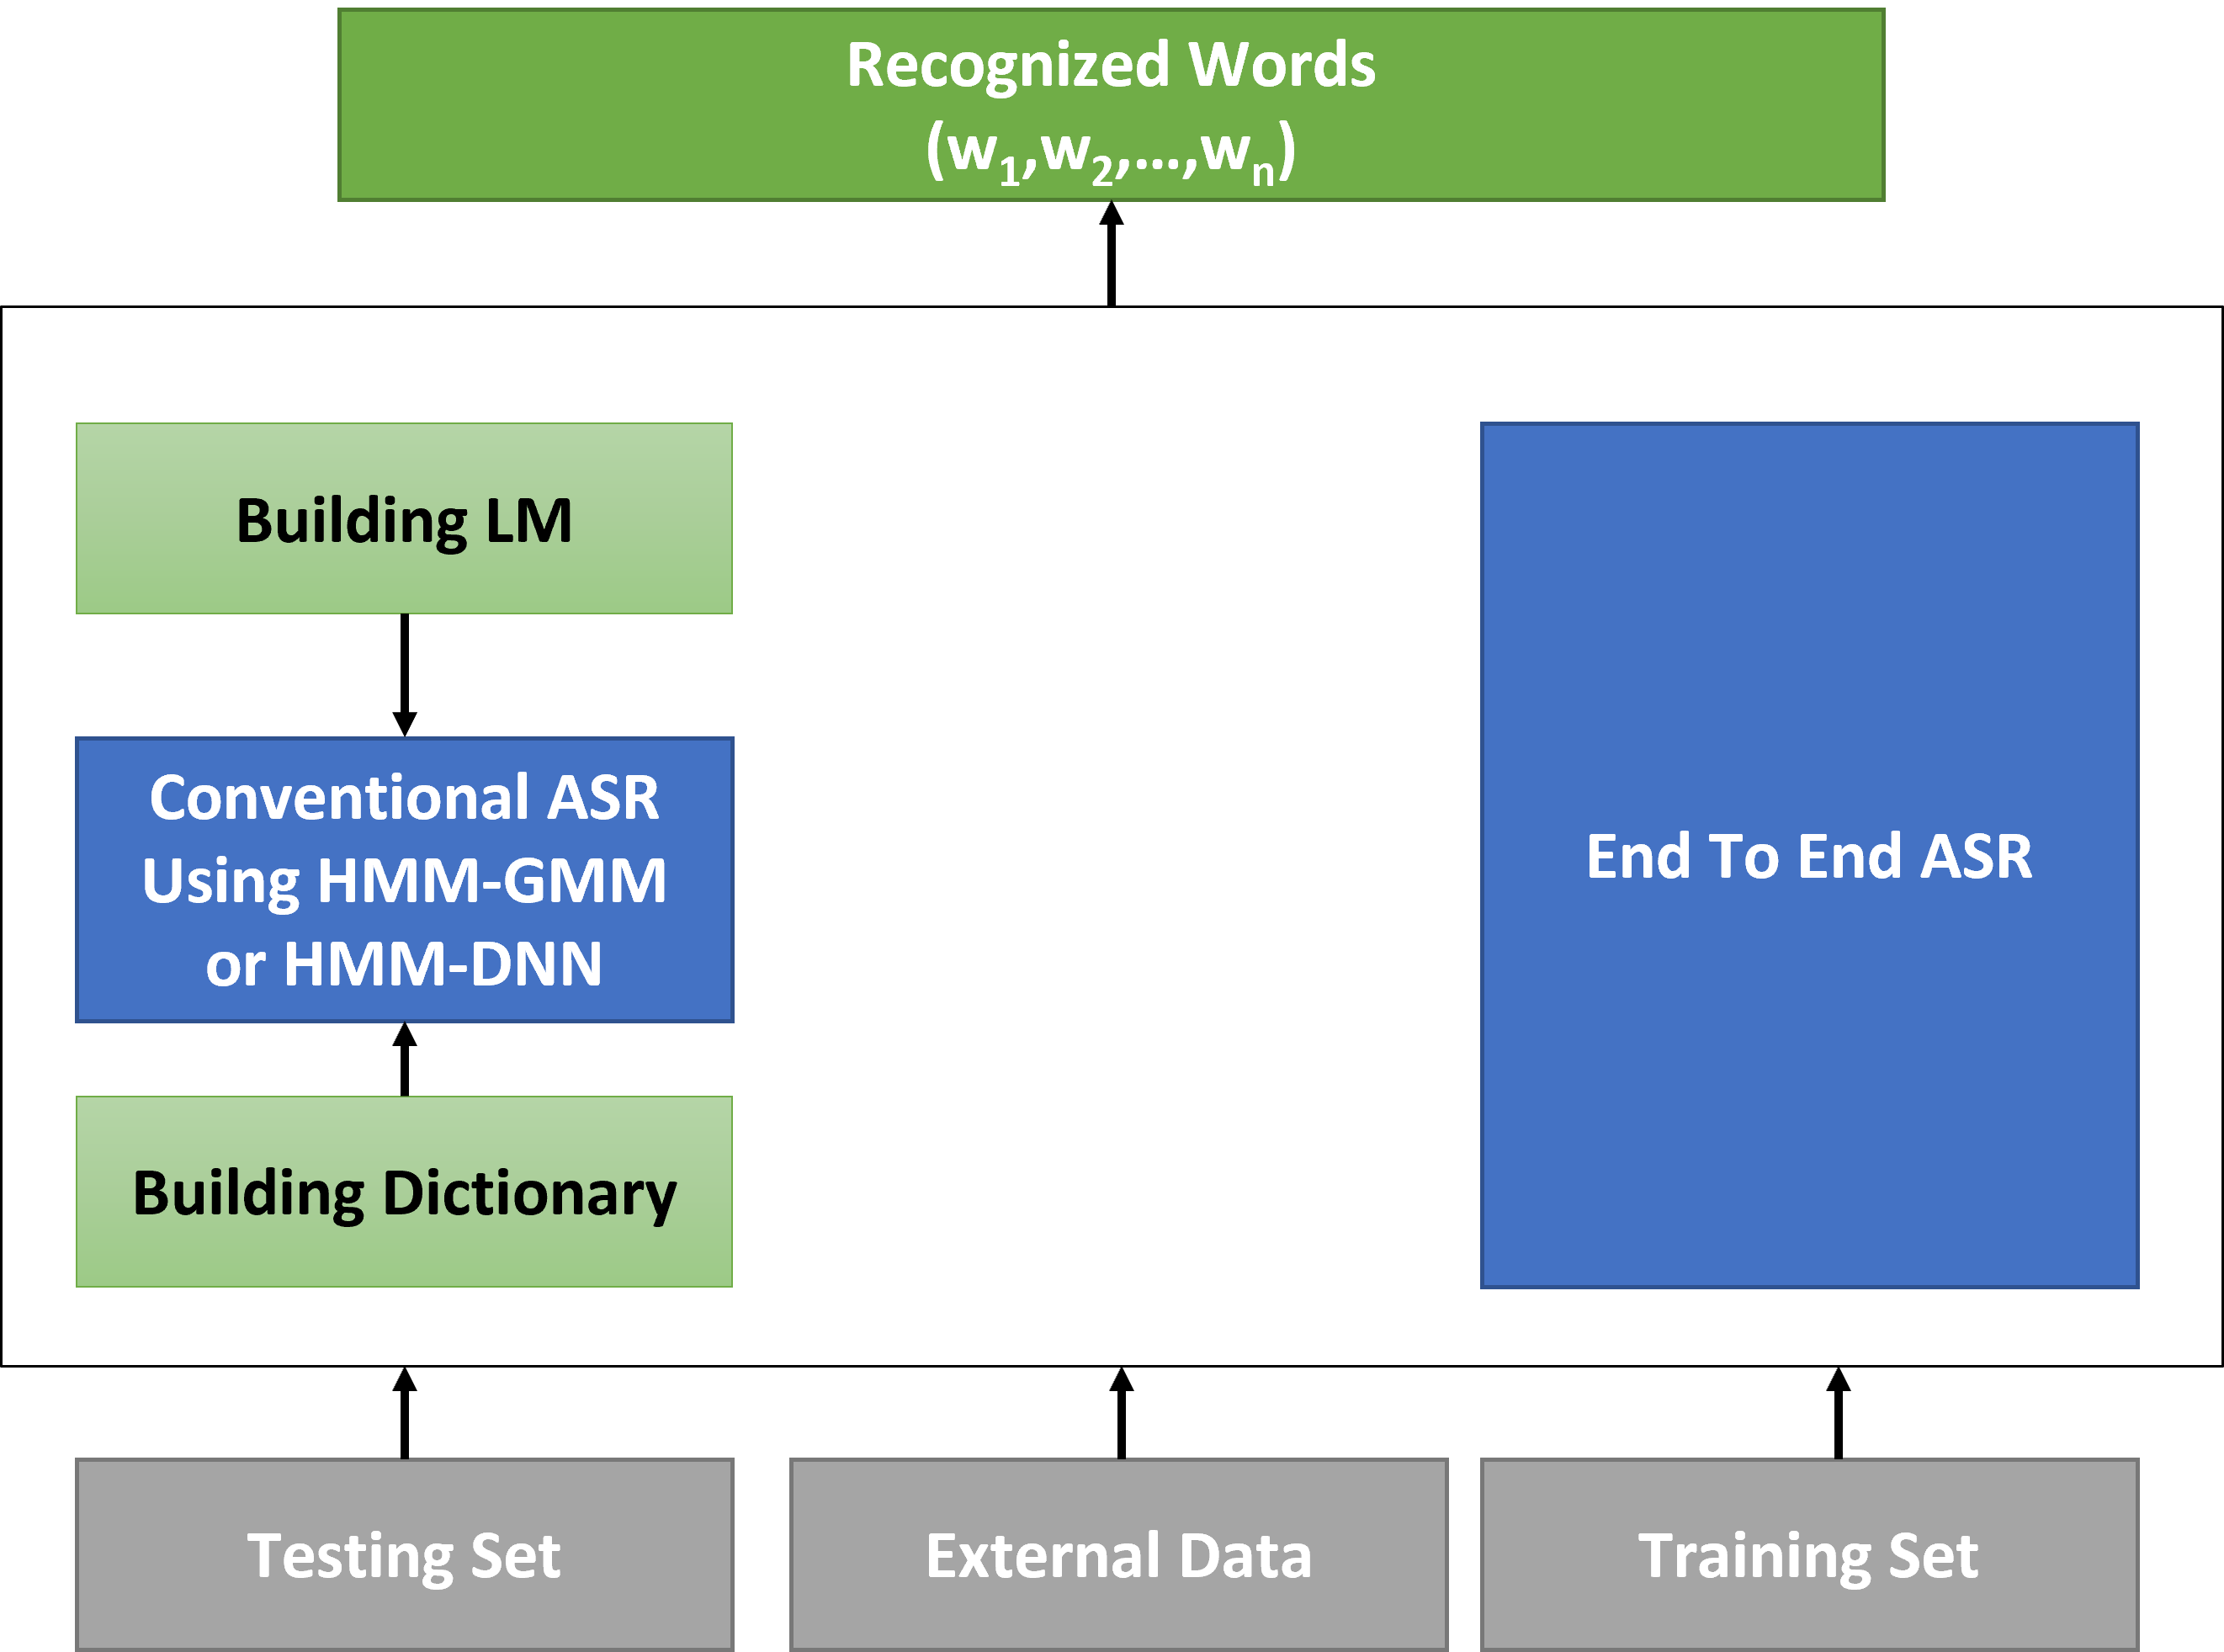
\includegraphics[width=0.4\textwidth]{img/E2EvsConventional.png}
    \caption{E2E ASR Architecture vs Conventional}
    \label{fig:e2e-asr}
\end{figure}

% E2E models utilize Deep Neural Networks like RNN \cite{sak_long_2014}, CNN \cite{abdel-hamid_exploring_2013}, TDNN \cite{kreyssig_improved_2018} and CNN-TDNN \cite{ghahremani_acoustic_2016}.

Due of the shortcomings of the Statistical HMM-based model and coupled with the promotion of deep learning technology, more and more works began to study end-to-end LVCSR. The goal was to bypass the complex structuring of Traditional ASR to achieve a joint language and acoustic model of sorts in one model using Deep Learning.

The E2E model \cite{eeckt_continual_2021} is a system that directly maps input audio sequence to sequence of words or other graphemes \cite{amodei_deep_2015-1, bell_adaptation_2020} using Deep Neural Networks like RNN \cite{sak_long_2014}, CNN \cite{abdel-hamid_exploring_2013}, TDNN \cite{kreyssig_improved_2018} and CNN-TDNN \cite{ghahremani_acoustic_2016}.

Despite its triumphs, the use of DNNs in speech processing has the following drawbacks \cite{backstrom_introduction_2022}:

\begin{itemize}
    \item DNN training on a specific dataset does necessarily improve the understanding of the problem. It's a black box because the model's reliability is not known. Although the design process gives some insights about languages, a trained speech recognizer on language "A" does not tell much about speech recognition on language "B" \cite{backstrom_introduction_2022}.
    \item DNN training is highly dependent on the data used to train it e.g. Models can be vulnerable to hidden biases, resulting in poor performance for OOVs or in a different scenario \cite{zhang_strategies_2019}.
    \item A trained DNN solves a specific problem, but does not tell how good the solution is. If a data set represents a circle in the 2D plane, that dataset can be accurately modelled with Sigmoids as non-linearities with a neural network. The neural network only needs to be large enough to handle the task at hand. The network, on the other hand, is several orders of magnitude more complex than the circle equation, which means that even though the network was successfully trained and the model is reasonably accurate, it gives no indication of whether the network's complexity is comparable to the problem's complexity \cite{backstrom_introduction_2022}.
    \item E2E models that are primarily DNN based typically require a large amount of training dataset, 1000 to 100,000 hours of speech to achieve peak performance. Such information is rarely available while also necessitating the purchase of costly hardware and computational resources \cite{kincaid_state_2018}.
    
\end{itemize}

To tackle these issues, the recent model design trend has been to return to classical design paradigms, in which models are based on a in-depth understanding of the problem, particularly in the case of Low-Resource Languages and the parameters of those models are then trained using ML methods \cite{backstrom_introduction_2022}. Advantages of using HMM-DNN models include:
\begin{itemize}
     \item It is a practical and effective method for ASR deployment on Low Computational Resources compared to Deep Learning Methods. 
     \item It takes less time to train in contrast to Deep Learning Methods \cite{naeem_subspace_2020}.
    \item Maintains the Structure that is required for a Language and Speech Processing System based on which the computer can understand the language better \cite{kincaid_state_2018}. Hence this works better in an environment where the context of speech is of the essence and has been applied for Continuous Speech Recognition as well \cite{backstrom_introduction_2022, morgan_continuous_1995}. 
    \item DNN-HMM can extend the labelling ability of GMM-HMM when the hidden layer and hidden unit numbers are set up properly in comparison to GMM-HMMs, shallow-NN-HMMs, and Multi-layer Perceptrons HMMs (MLPHMMs). Thus, DNN-HMMs with discriminative pre-training can produce good results in our scenario as well \cite{li_hybrid_2013}.
    \item HMM–DNN (especially TDNN) is streamable while E2E-transformer is not \cite{ritter_neural_2019}. 
    \item Computationally intensive compared to E2E Systems \cite{kincaid_brief_2018}.
    \item E2E modelling is less mature than hybrid modelling, and much of the research on E2E modelling is focused on improving general modelling technology \cite{backstrom_introduction_2022}. 
    \item Easily models correlated features like spectral features and input context includes multiple data-frames at input \cite{backstrom_introduction_2022}. 
    \item Because E2E models typically contain sub-networks corresponding to the acoustic model and language model in hybrid models, most adaptation technologies successfully applied to hybrid models by adapting acoustic model or language model can also work well for E2E models \cite{backstrom_introduction_2022}. %Most adaptation technologies successfully applied to hybrid models by adapting acoustic model or language model can also work well for E2E models \cite{backstrom_introduction_2022} since E2E models typically contain sub-networks corresponding to the acoustic model and language model in hybrid models.
    \item Greater flexibility than GMMs because it is not made of nearly local components since GMMs are inefficient for non-linear class boundaries \cite{bell_adaptation_2021}.
    \item NNs can simultaneously model multiple events in the input compared to GMMs, i.e. different sets of hidden units modelling each event, whereas GMMs assume generation of each from by a single mixture component \cite{hussein_arabic_2022}.
    \item NNs can learn more complex representations compared to GMMs and higher-level features such as tandem, posteriorgrams, bottleneck features (like in TDNN) etc \cite{liu_time_2019}.
    \item Components in hybrid HMM-DNN models are optimised separately, whereas E2E models use a single objective function which is why E2E models tend to memorise the training data more, making generalisation or robustness to unseen data difficult for E2E models. Thus, adaptation to a new environment or domain is critical to the large-scale application of E2E models \cite{backstrom_introduction_2022}. 
\end{itemize}

However, HMM–DNN models have some drawbacks like model complexity i.e. complicated to implement since it deploys a modular design, separately training different modules for acoustic modeling, pronunciation lexicon, and language modeling,  requiring of linguistic resources \cite{hussein_arabic_2022}. But as a trade-off for performance, data-set and computation requirement, in our scenario, Using HMM-DNN makes the most sense \cite{georgescu_performance_2021}.

\subsection{TDNN}

\begin{figure}[htb]
    \centering
    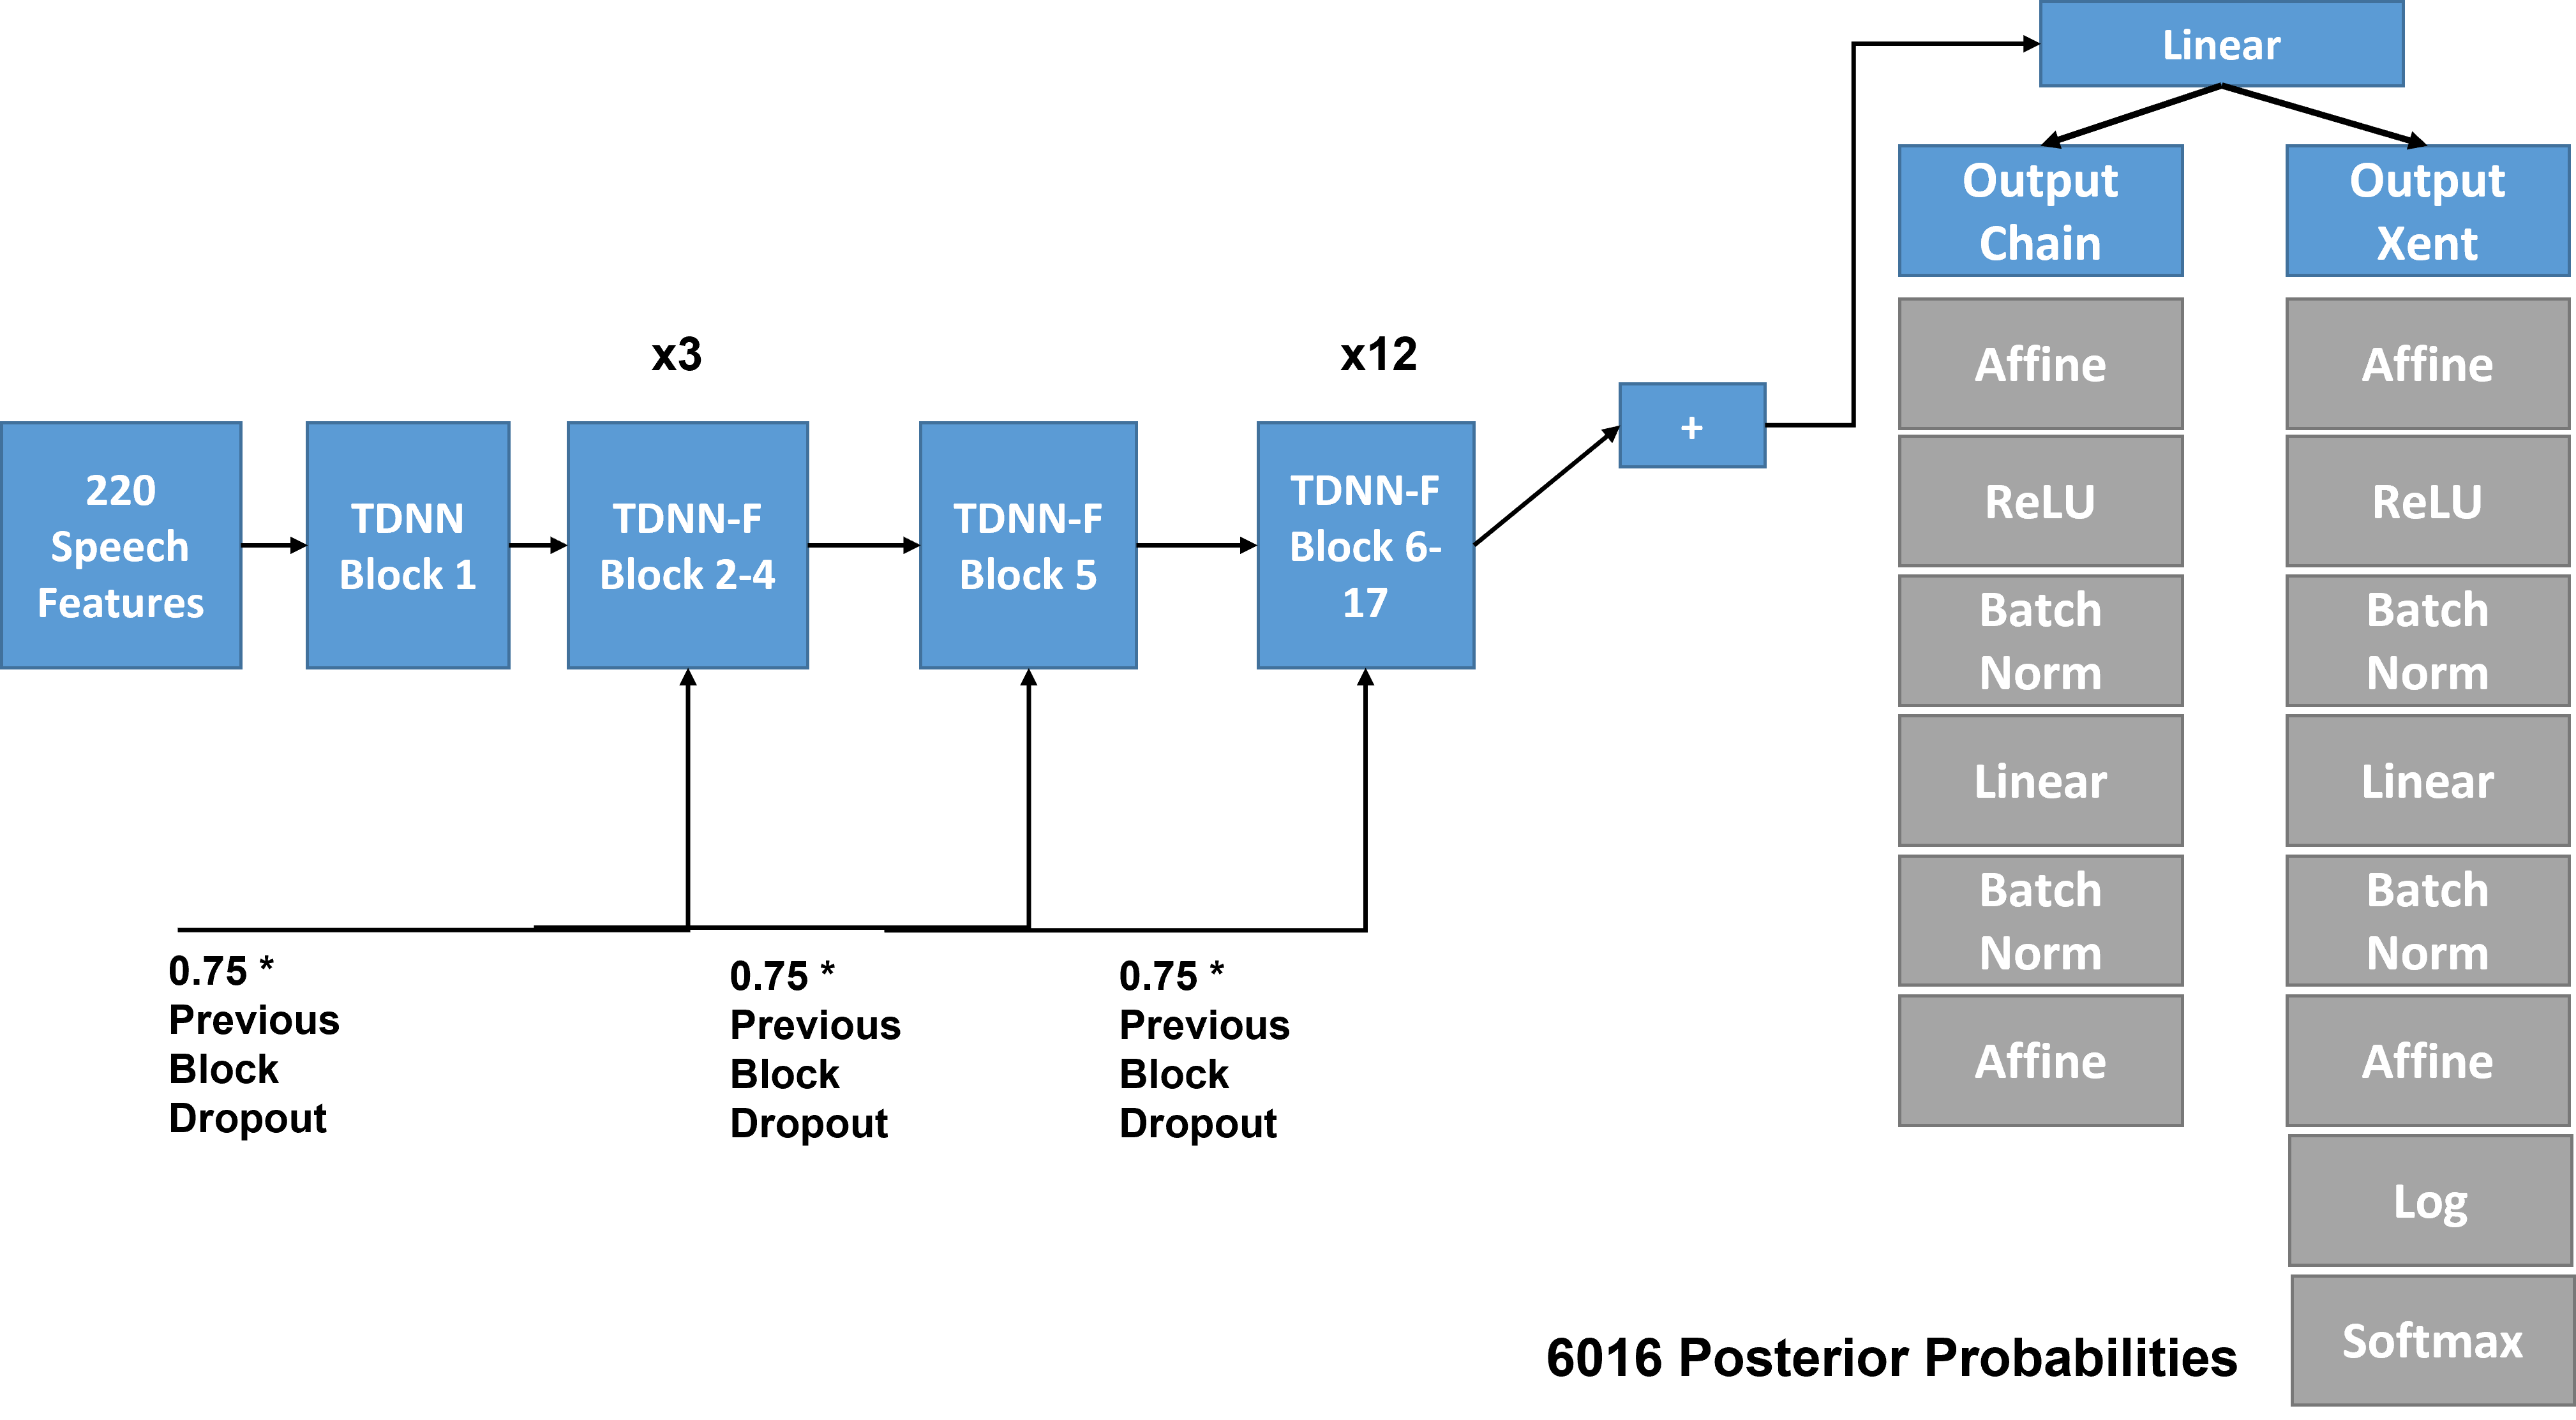
\includegraphics[width=0.40\textwidth]{img/TDNN2.png}
    \caption{TDNN Architecture Basic Layout}
    \label{fig:TDNN-arch}
\end{figure}

Time-Delay Neural Network (TDNN), originally invented by Alex Waibel and Geoffrey Hinton, captures long term temporal correlations between speech frames i.e they are time-dilated 1-Dimensional CNNs. It is a time-domain convolutional network that models temporal dependencies which is easier to parallelize in contrast to a recurrent network and is comparable to feed-forward DNN in terms of training time \cite{noauthor_tdnn_nodate}. It has special characteristics of shift in-variance just like CNN. TDNN can learn short intervals contexts between input features like MFCC and of longer intervals in upper layers i.e. lower layers learn short input contexts, and higher layers learn long input contexts \cite{liu_time_2019}.

\begin{figure}[h!]
    \centering
    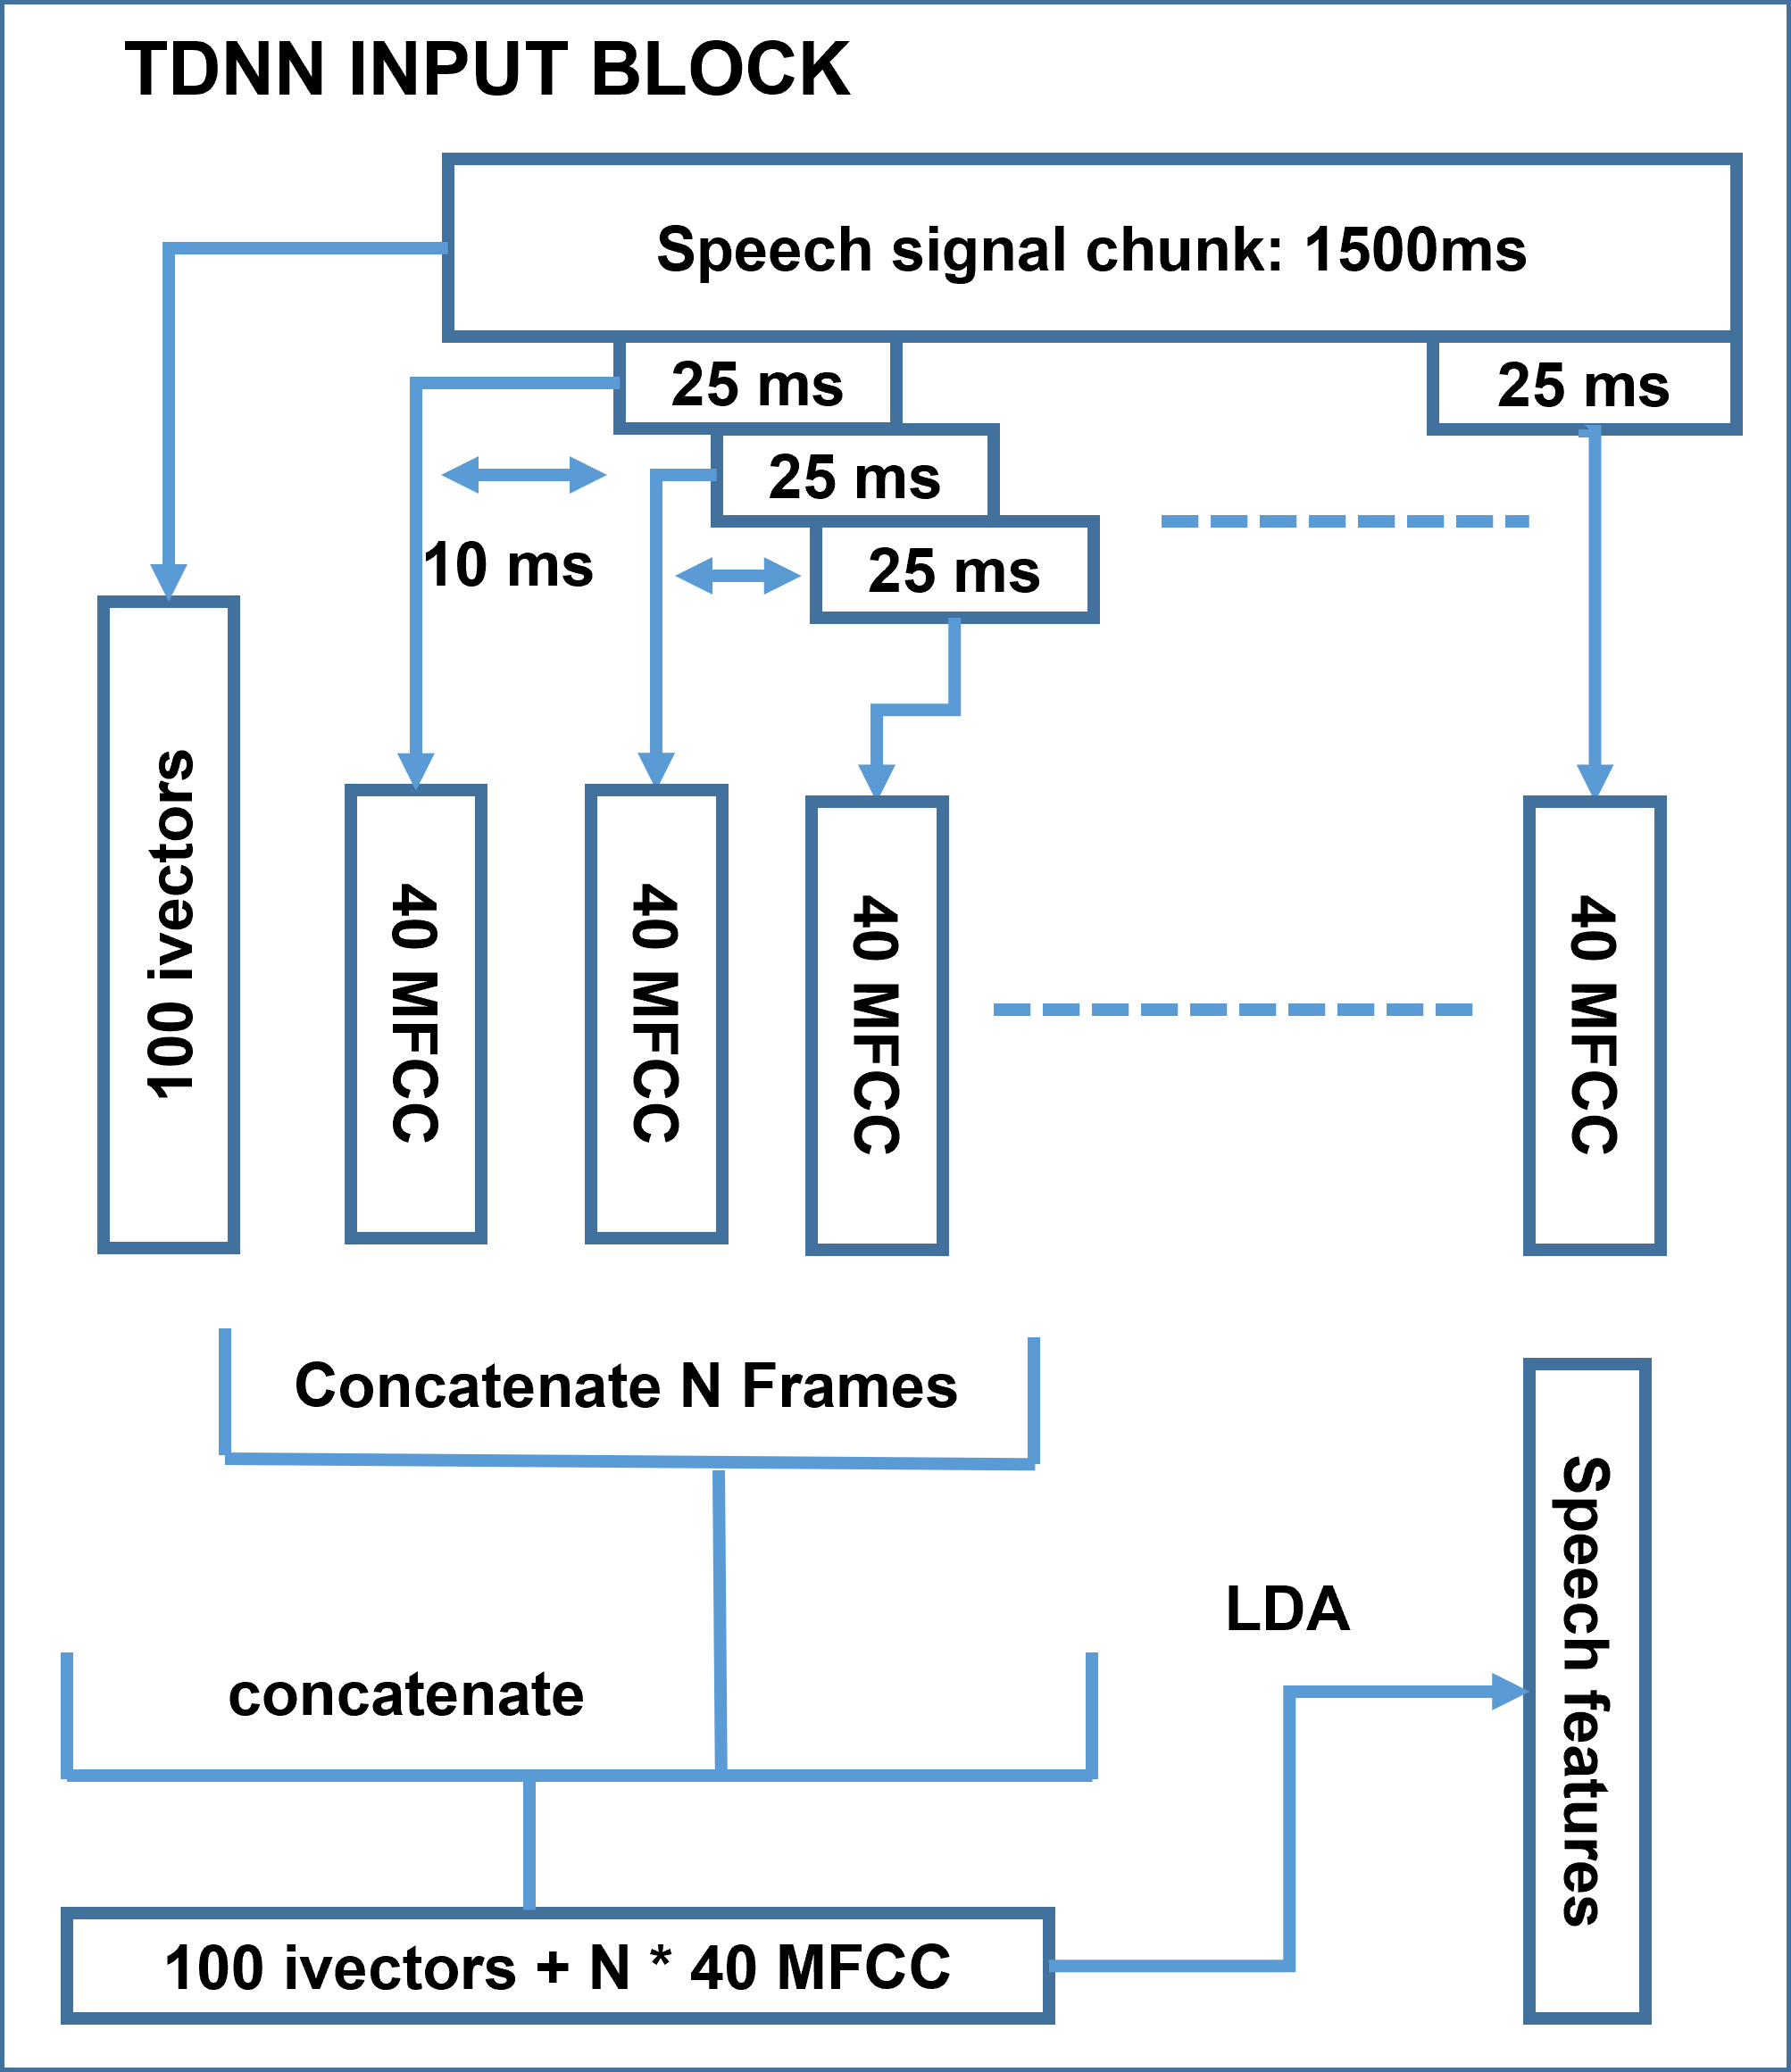
\includegraphics[width=0.2\textwidth]{img/TDNN INPUT.png}
    %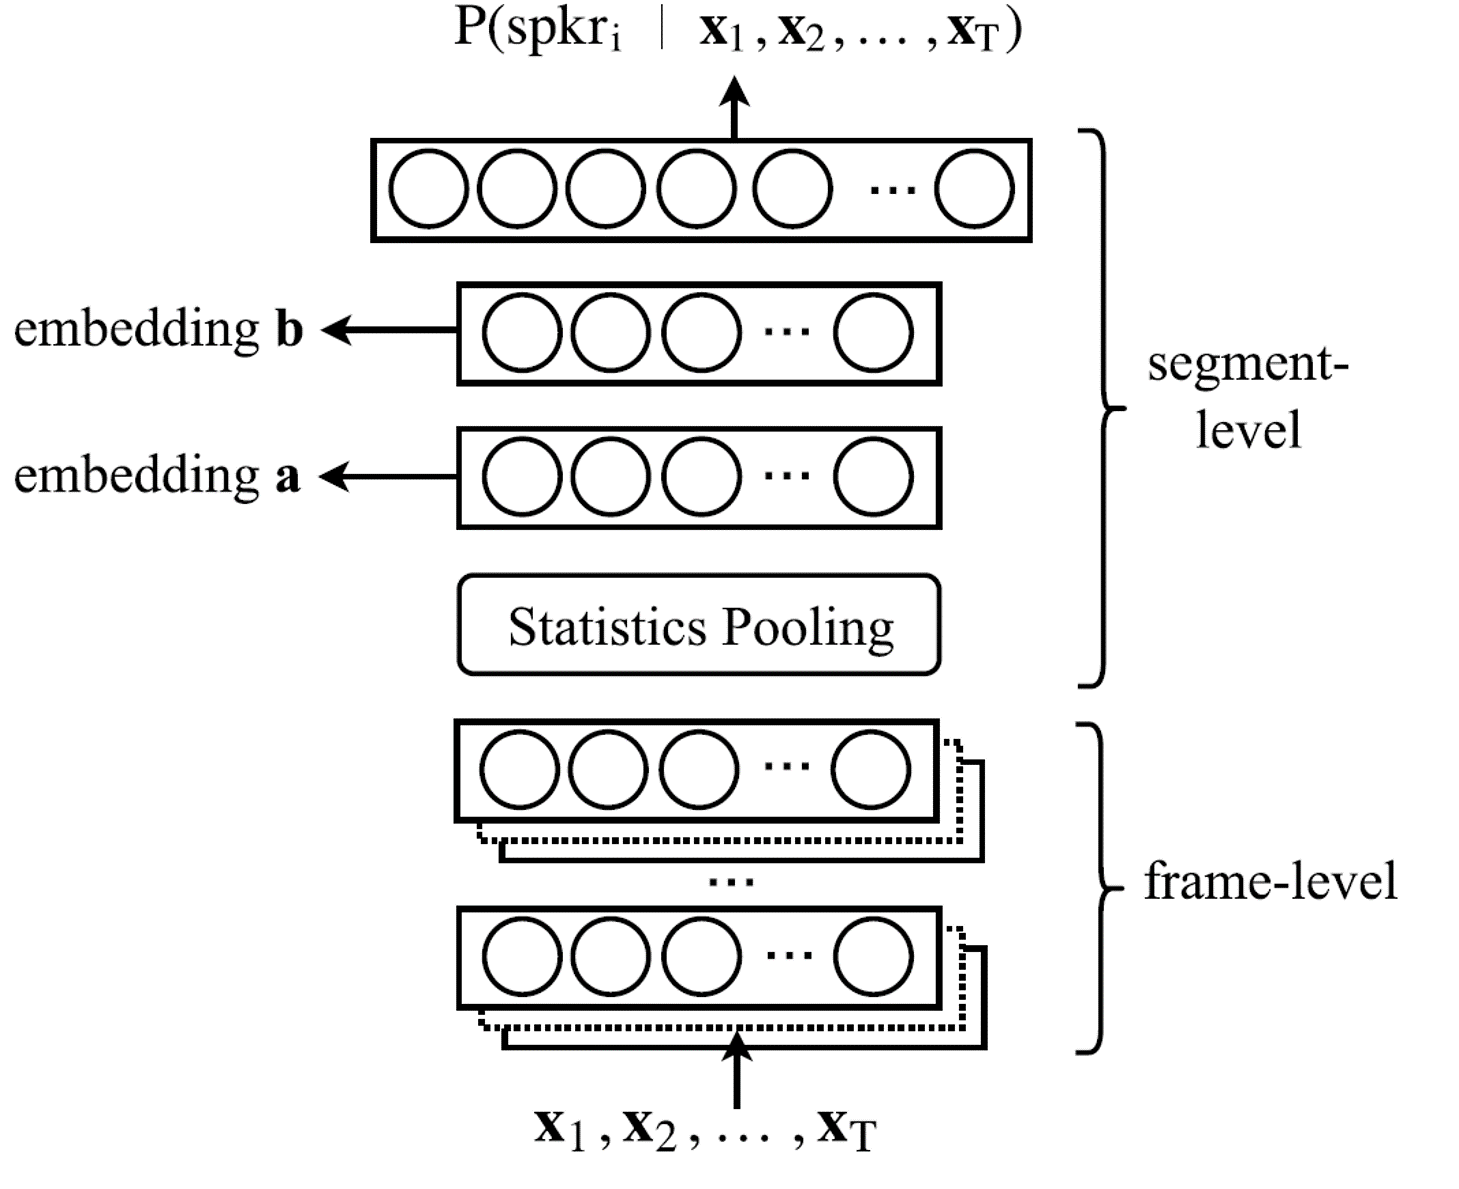
\includegraphics[width=0.4\textwidth]{img/tdDNN frame and segment.png}
    \caption{TDNN Input}   
    \label{fig:TDNN-INPUT}
\end{figure}

Each unit's input is spatially expanded out in a couple of sequential units from the previous TDNN layer. Hence, the lower layers learn a narrow-context and higher layers process a broader temporal-context activations. Each layer's input-context length represents the TDNN hyperparameter \cite{kreyssig_improved_2018}.

All features and frames are correlated in speech. We simply make a 25ms window and take 40 MFCCs of that window or segment. We need previous and next frames to predict next frame in actual. In streaming where we want to predict more on based on past frames instead of future frames, TDNN make better sense \cite{liu_time_2019}. 

\begin{figure}[h!]
    \centering
    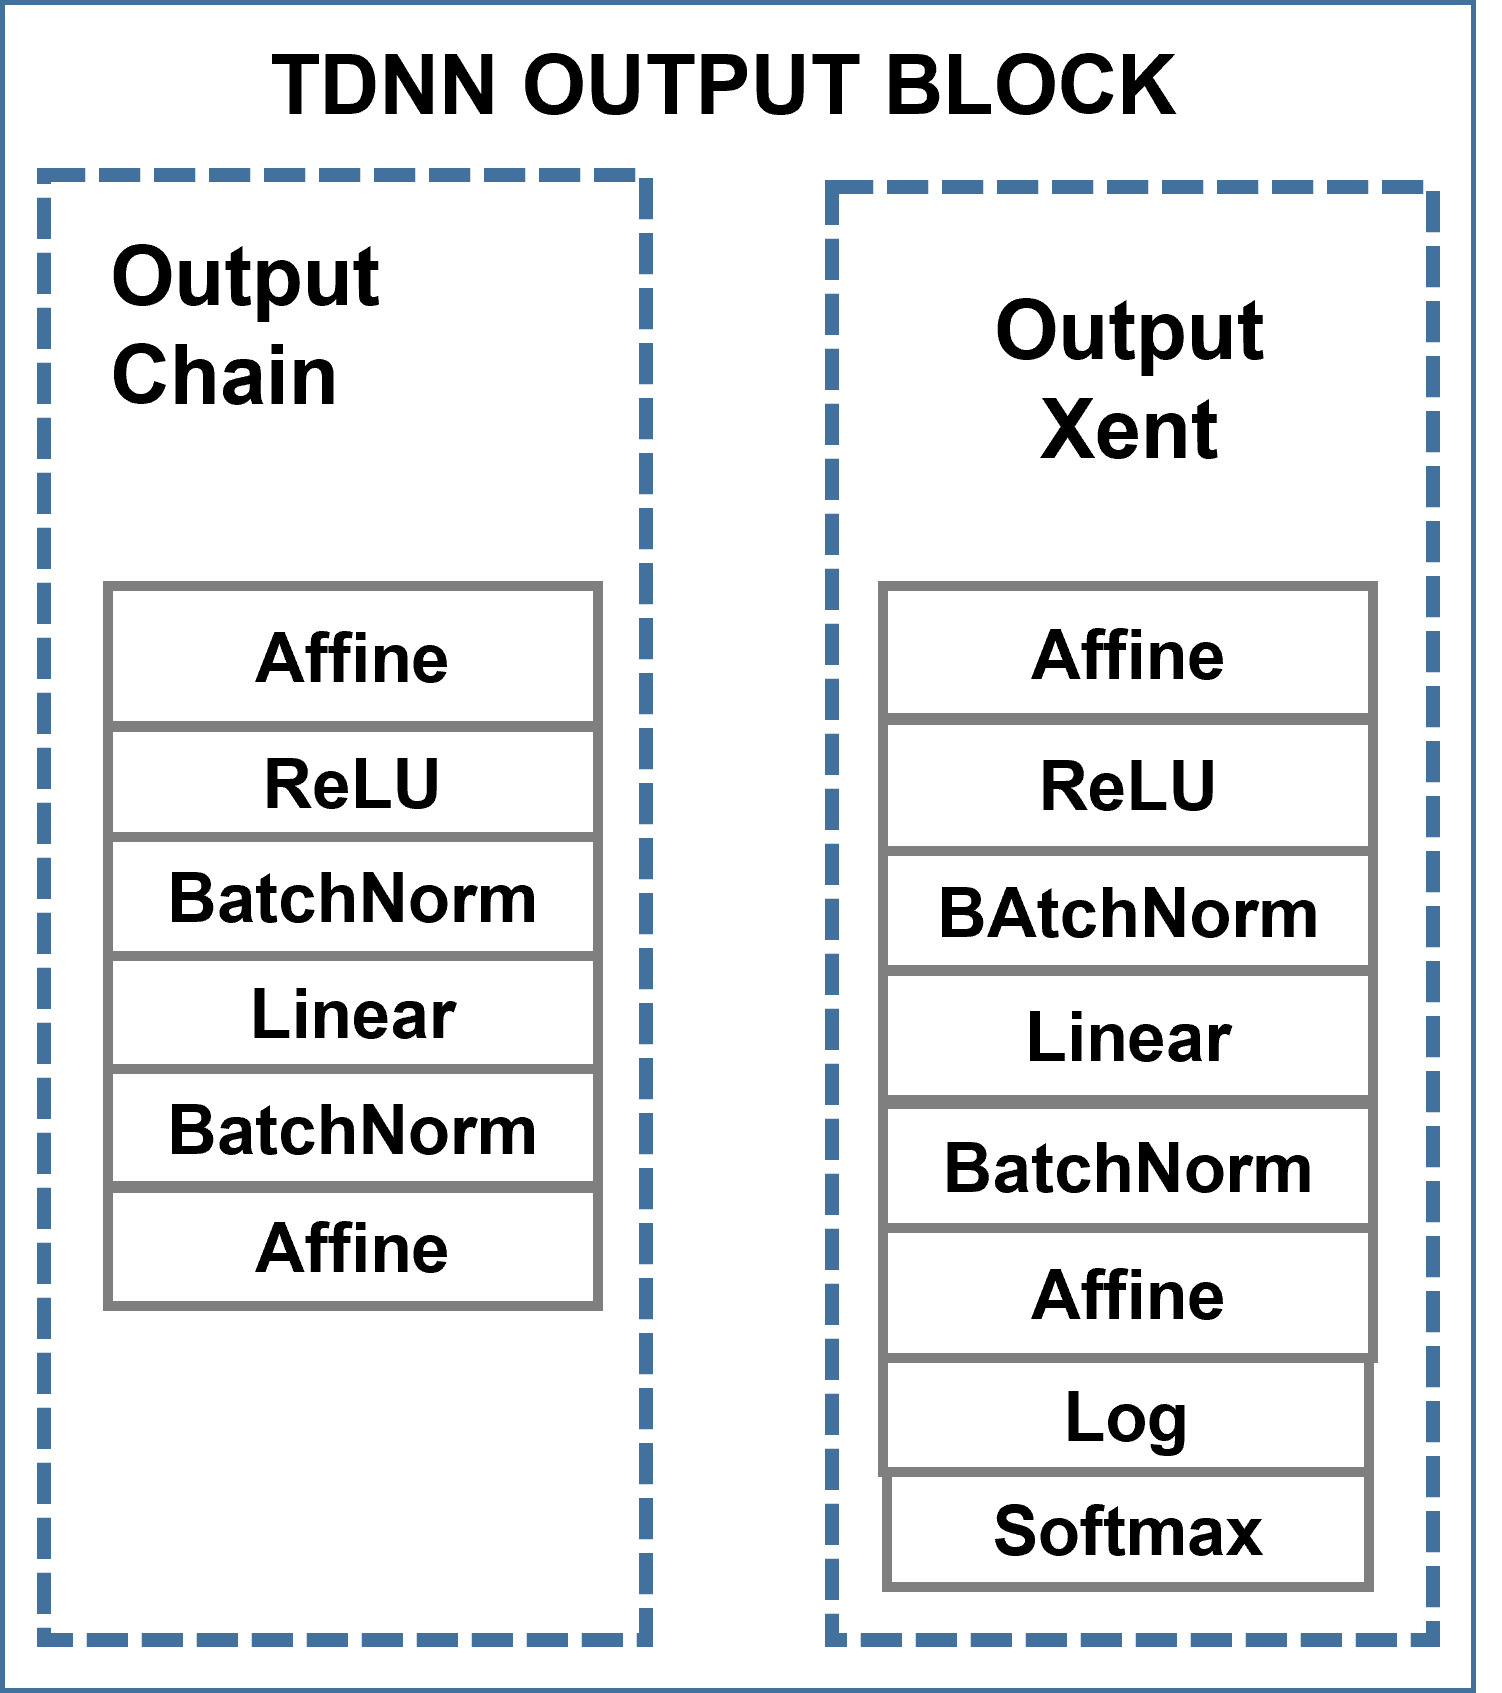
\includegraphics[width=0.3\textwidth]{img/TDNNOUTPUT.png}
    \caption{TDNN Output Block}
    \label{fig:TDNN-OUTPUT-BLOC}
\end{figure}

%\begin{figure}[h!]
%    \centering
%    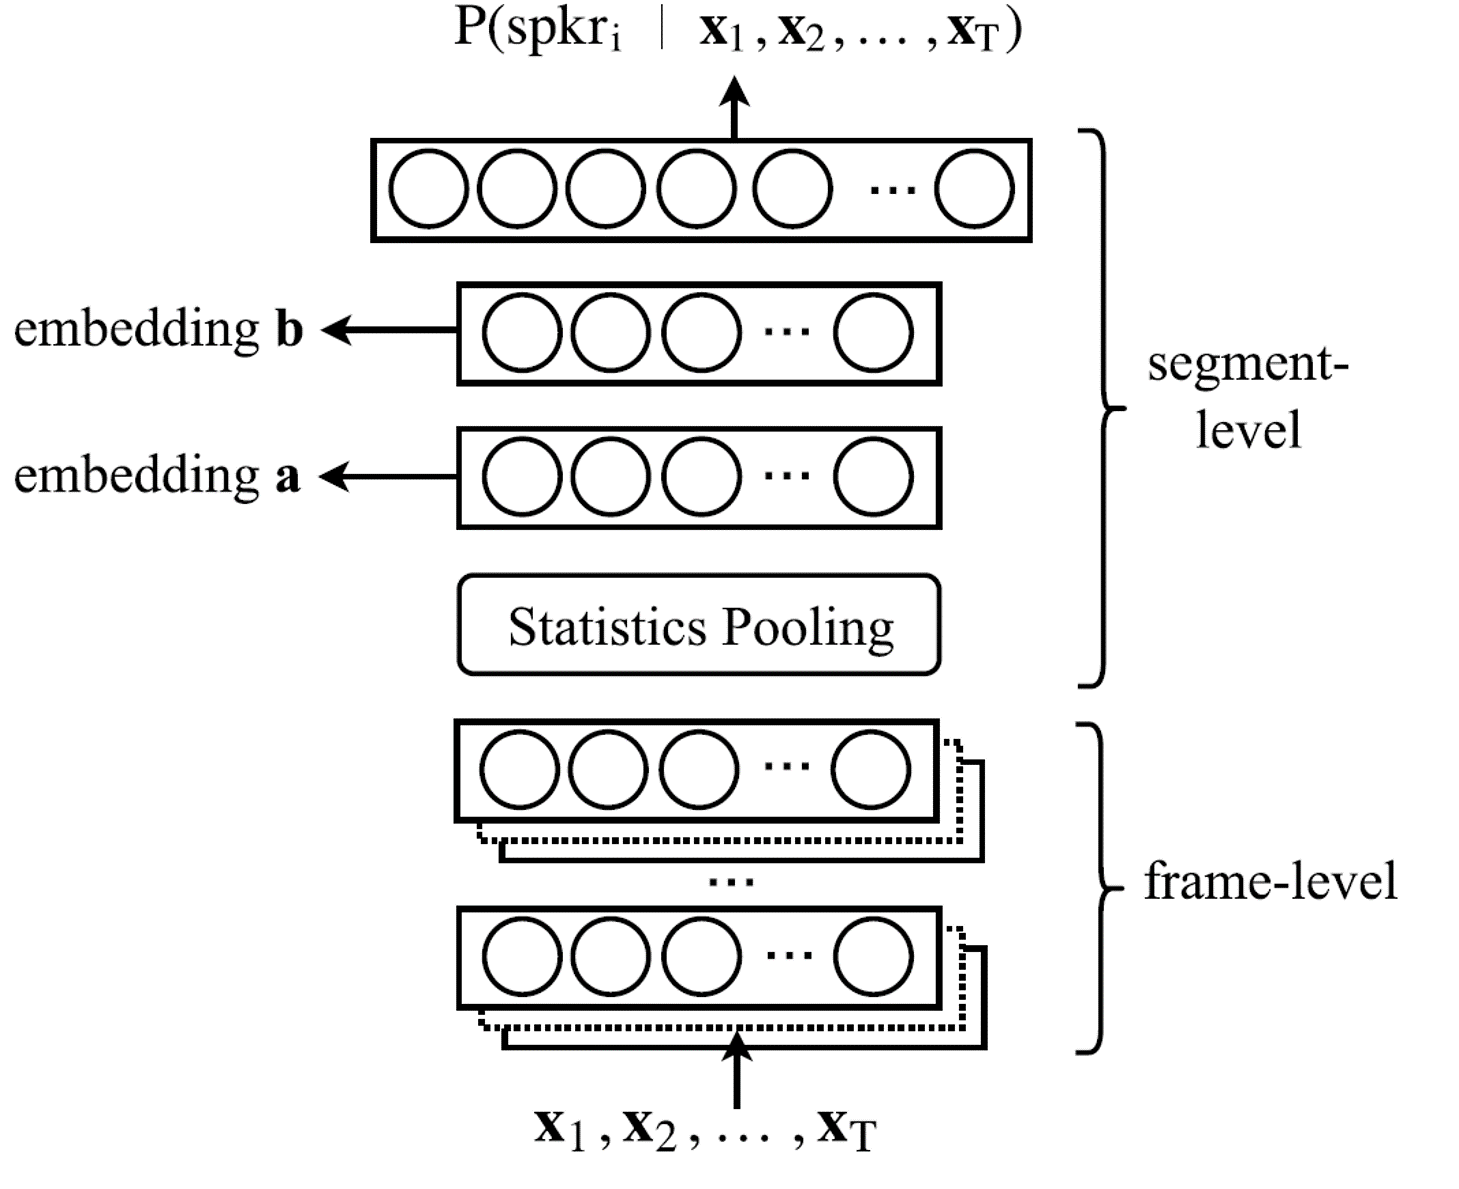
\includegraphics[width=0.5\textwidth]{img/tdDNN frame and segment.png}
%    \caption{TDNN Layers at frame and segment level}
%    \label{fig:TDNN Layers}
%\end{figure}

Input patches consist of fixed number of feature vectors as input to which processes them with fixed local temporal context. The context width increases as we go to upper layers. Finally the last layer representation is pooled by statistics pool layer. The network consist of TDNN which operates at frame level. The last layer output representations from TDNN goes to Statistics pooling layer at every time step. Statistic pool layer computes mean and standard vectors for all the representations from frame 1 to T. Finally these pooled representation goes to next layer which applies affine transformation followed by softmax which can be used for Speech to text of identifying speakers \cite{liu_time_2019}. 

The TDNN architecture is learned on narrow contexts and the upper layers of the networks process wider contexts of the input features, whereas the general Feed Forward Neural Network learns entire input features for processing contexts. Each TDNN layer is updated by a different resolution, which increases as the network layers. By removing duplicated weights from the networks, the TDNN is optimised. A standard Feed Forward Neural learns overlapping features, and removing these duplicated updates reduces training time \cite{yeh_taiwanese_2020}. 

A subsampling is used to reduce duplicated inputs as shown in \ref{fig:tdnn-subsampling} in which nodes and weights (shown by dashed line) are updated only upon application of sub-sampling. The technique does not connect multiple inputs in a hidden layer by allowing space between frames. Since TDNN has a long context going up to the upper layer, the model can learn all input features if the interval between frames is allowed \cite{ritter_neural_2019}. 

\begin{figure}[h!]
    \centering
    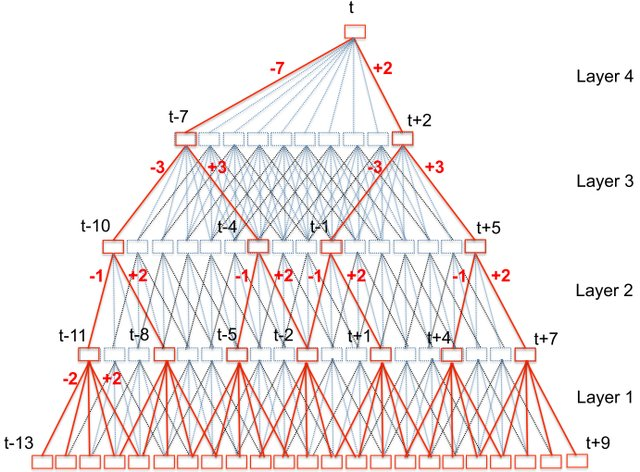
\includegraphics[width=0.40\textwidth]{img/Tdnn-subsampling.jpg}
    \caption{TDNN subsampling \cite{ritter_neural_2019}}
    \label{fig:tdnn-subsampling}
\end{figure}

Furthermore, minimizing the number of edges and nodes in the network reduces the number of parameters that represent the model. Long-term temporal dependencies are better captured by TDNN architecture than by feed-forward DNN. In comparison to baseline DNN model in interactive personal assistant (IPA) domain there is a relative improvement of 7.3\%.  The TDNN is also used to remove reverberation effects in robust acoustic modelling. Using iVectors as input helps TDNN to perform instantaneous speaker and environment adaptation potentially improving 10\% WER \cite{yeh_taiwanese_2020}.

Increasing TDNN layers enables the network to capture features for a longer time period. Deepening the number of network layers of TDNN helps yield better results. However, deeper network tends to cause degradation, hence, the increasing depth of the neural network reduces accuracy for which a different TDNN architecture is used  in order to achieve better speech recognition performance in which Matrix Factorization training of the network makes neural network training stable \cite{povey_semi-orthogonal_2018}.

\subsection{CNN-TDNN}

CNN-TDNN \cite{ghahremani_acoustic_2016} is a variant of simple TDNN model and it is part of a multi-component system comprising of a hybrid HMM-TDNN based acoustic, phonetic and n-gram language model. It has CNN blocks before the TDNN blocks and takes Mel Filterbanks as input instead of MFCCs. The detailed working of this model is given in Section \ref{sec:LFMMI-chain}

\begin{figure}[htb]
    \centering
    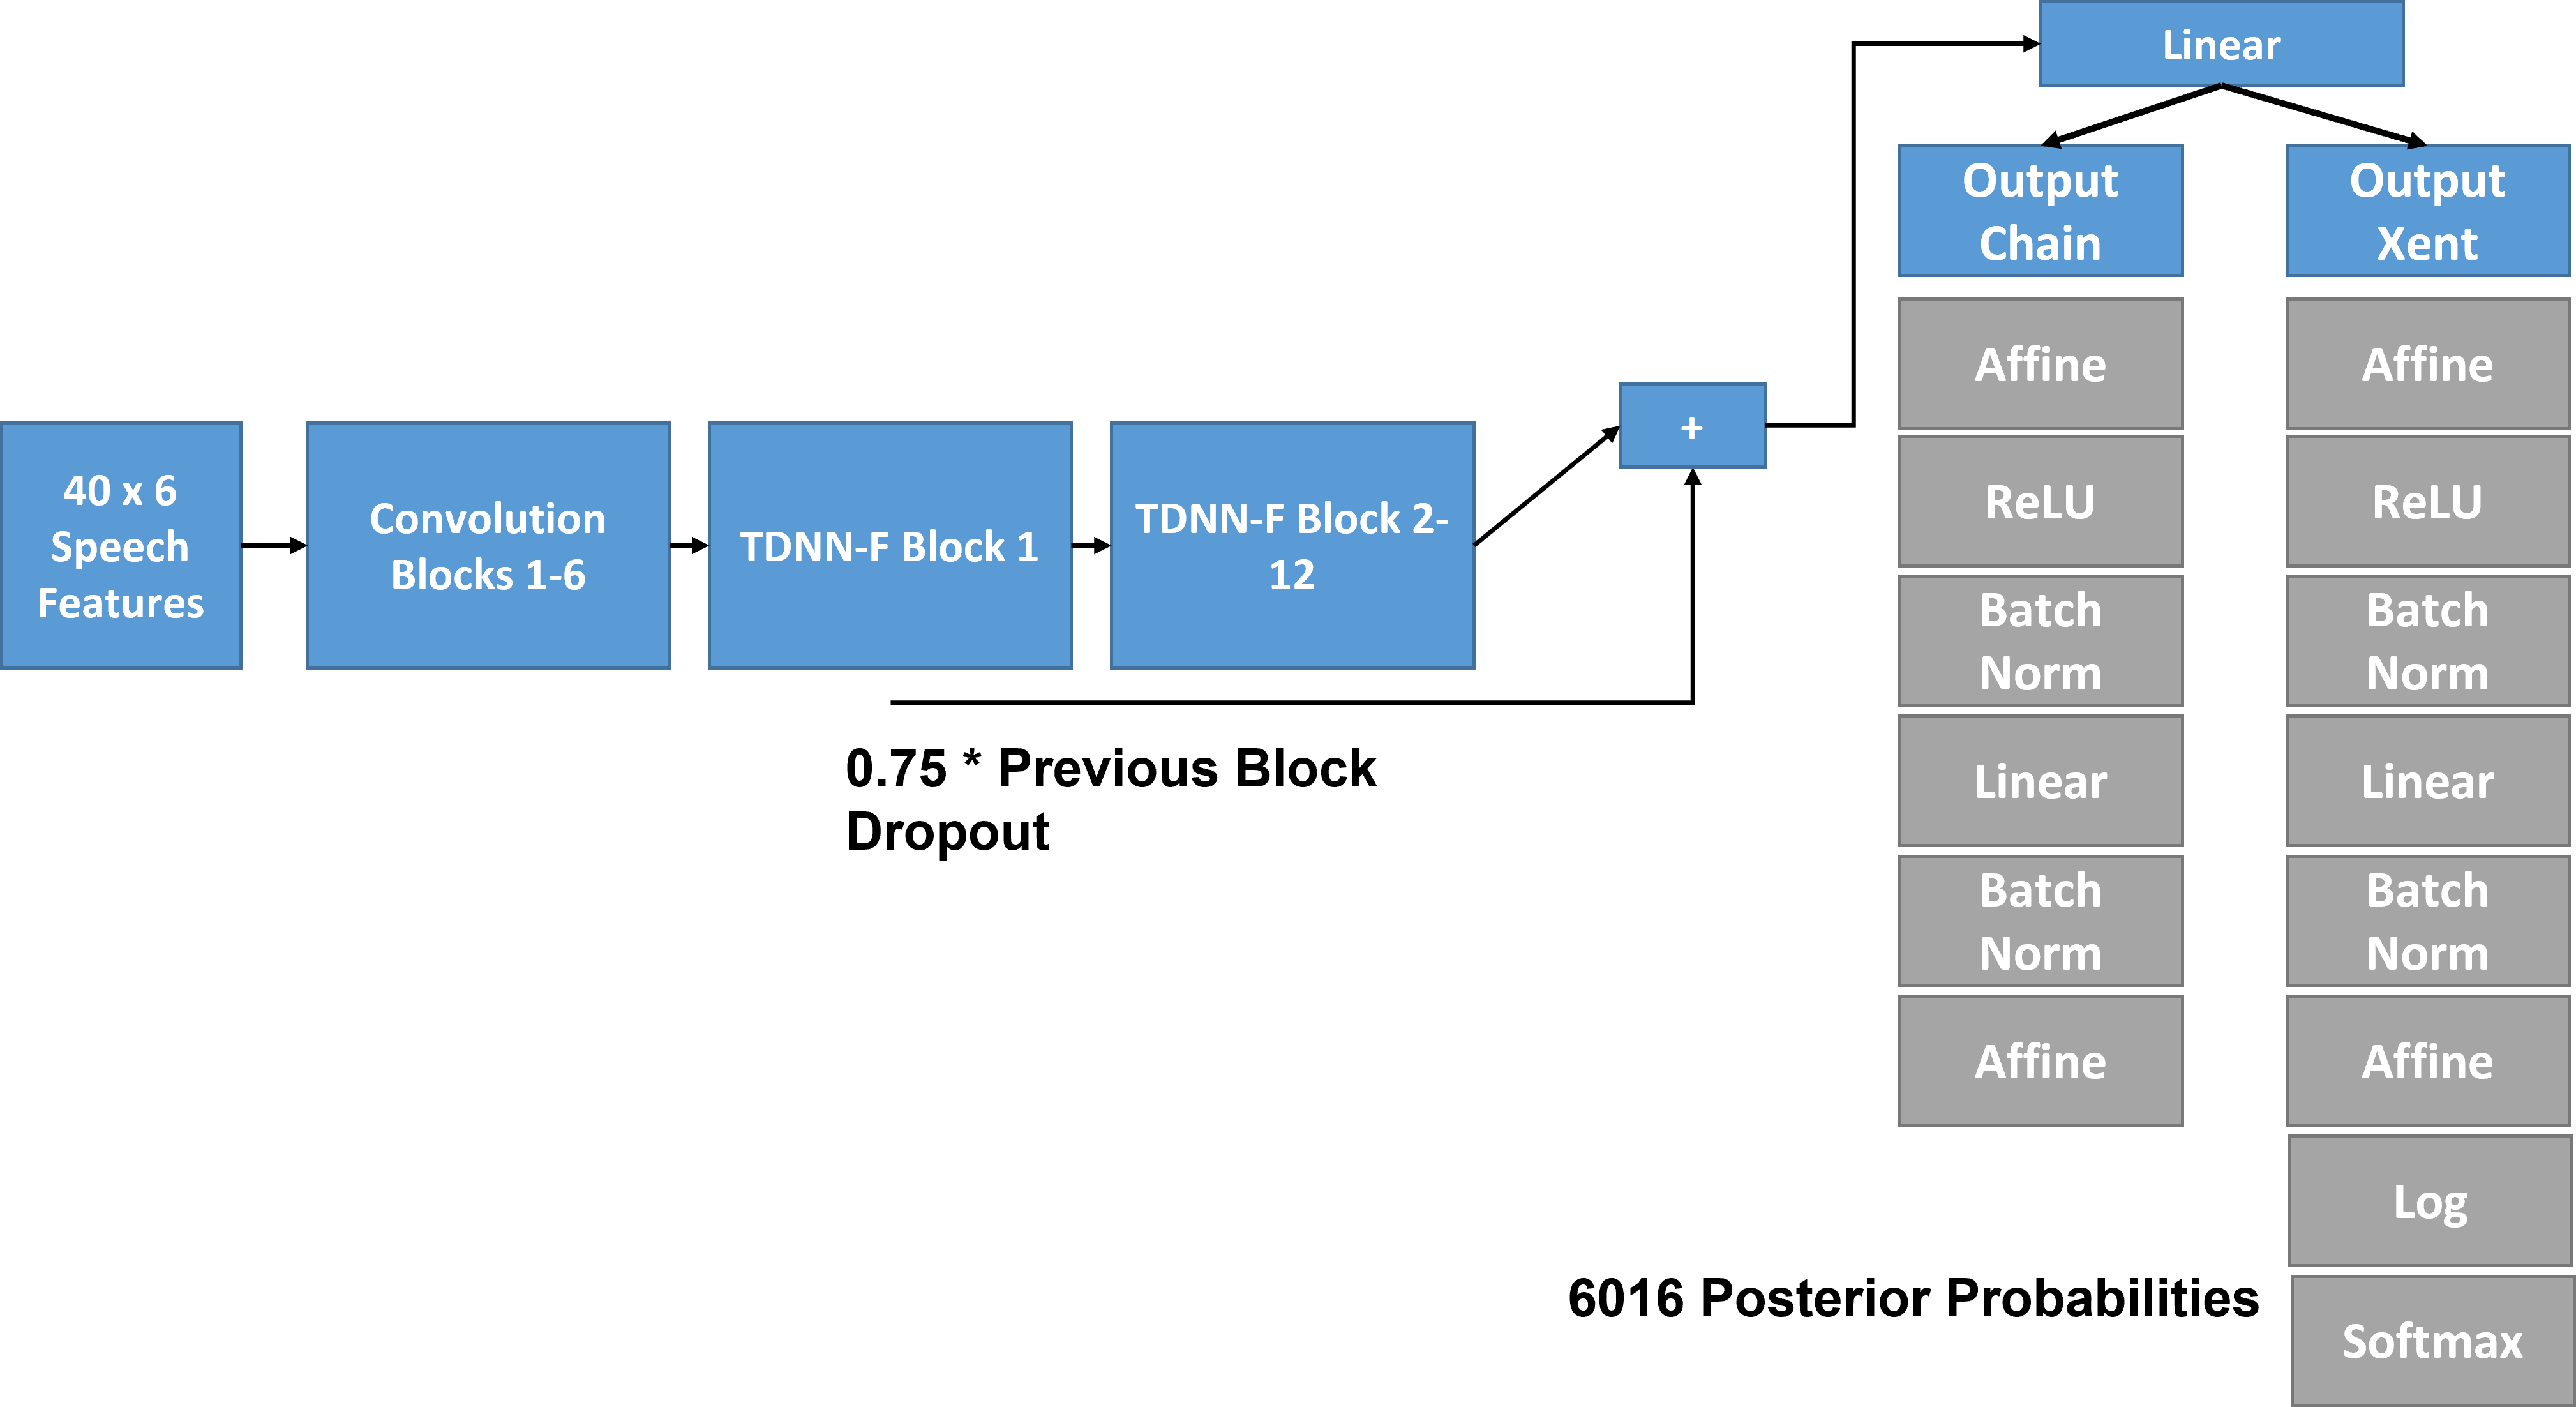
\includegraphics[width=0.45\textwidth]{img/CNNTDNN2.png}
    \caption{CNN-TDNN Basic Layout}
    \label{fig:CNNTDNN-Layout}
\end{figure}

\begin{figure}[h!]
    \centering
    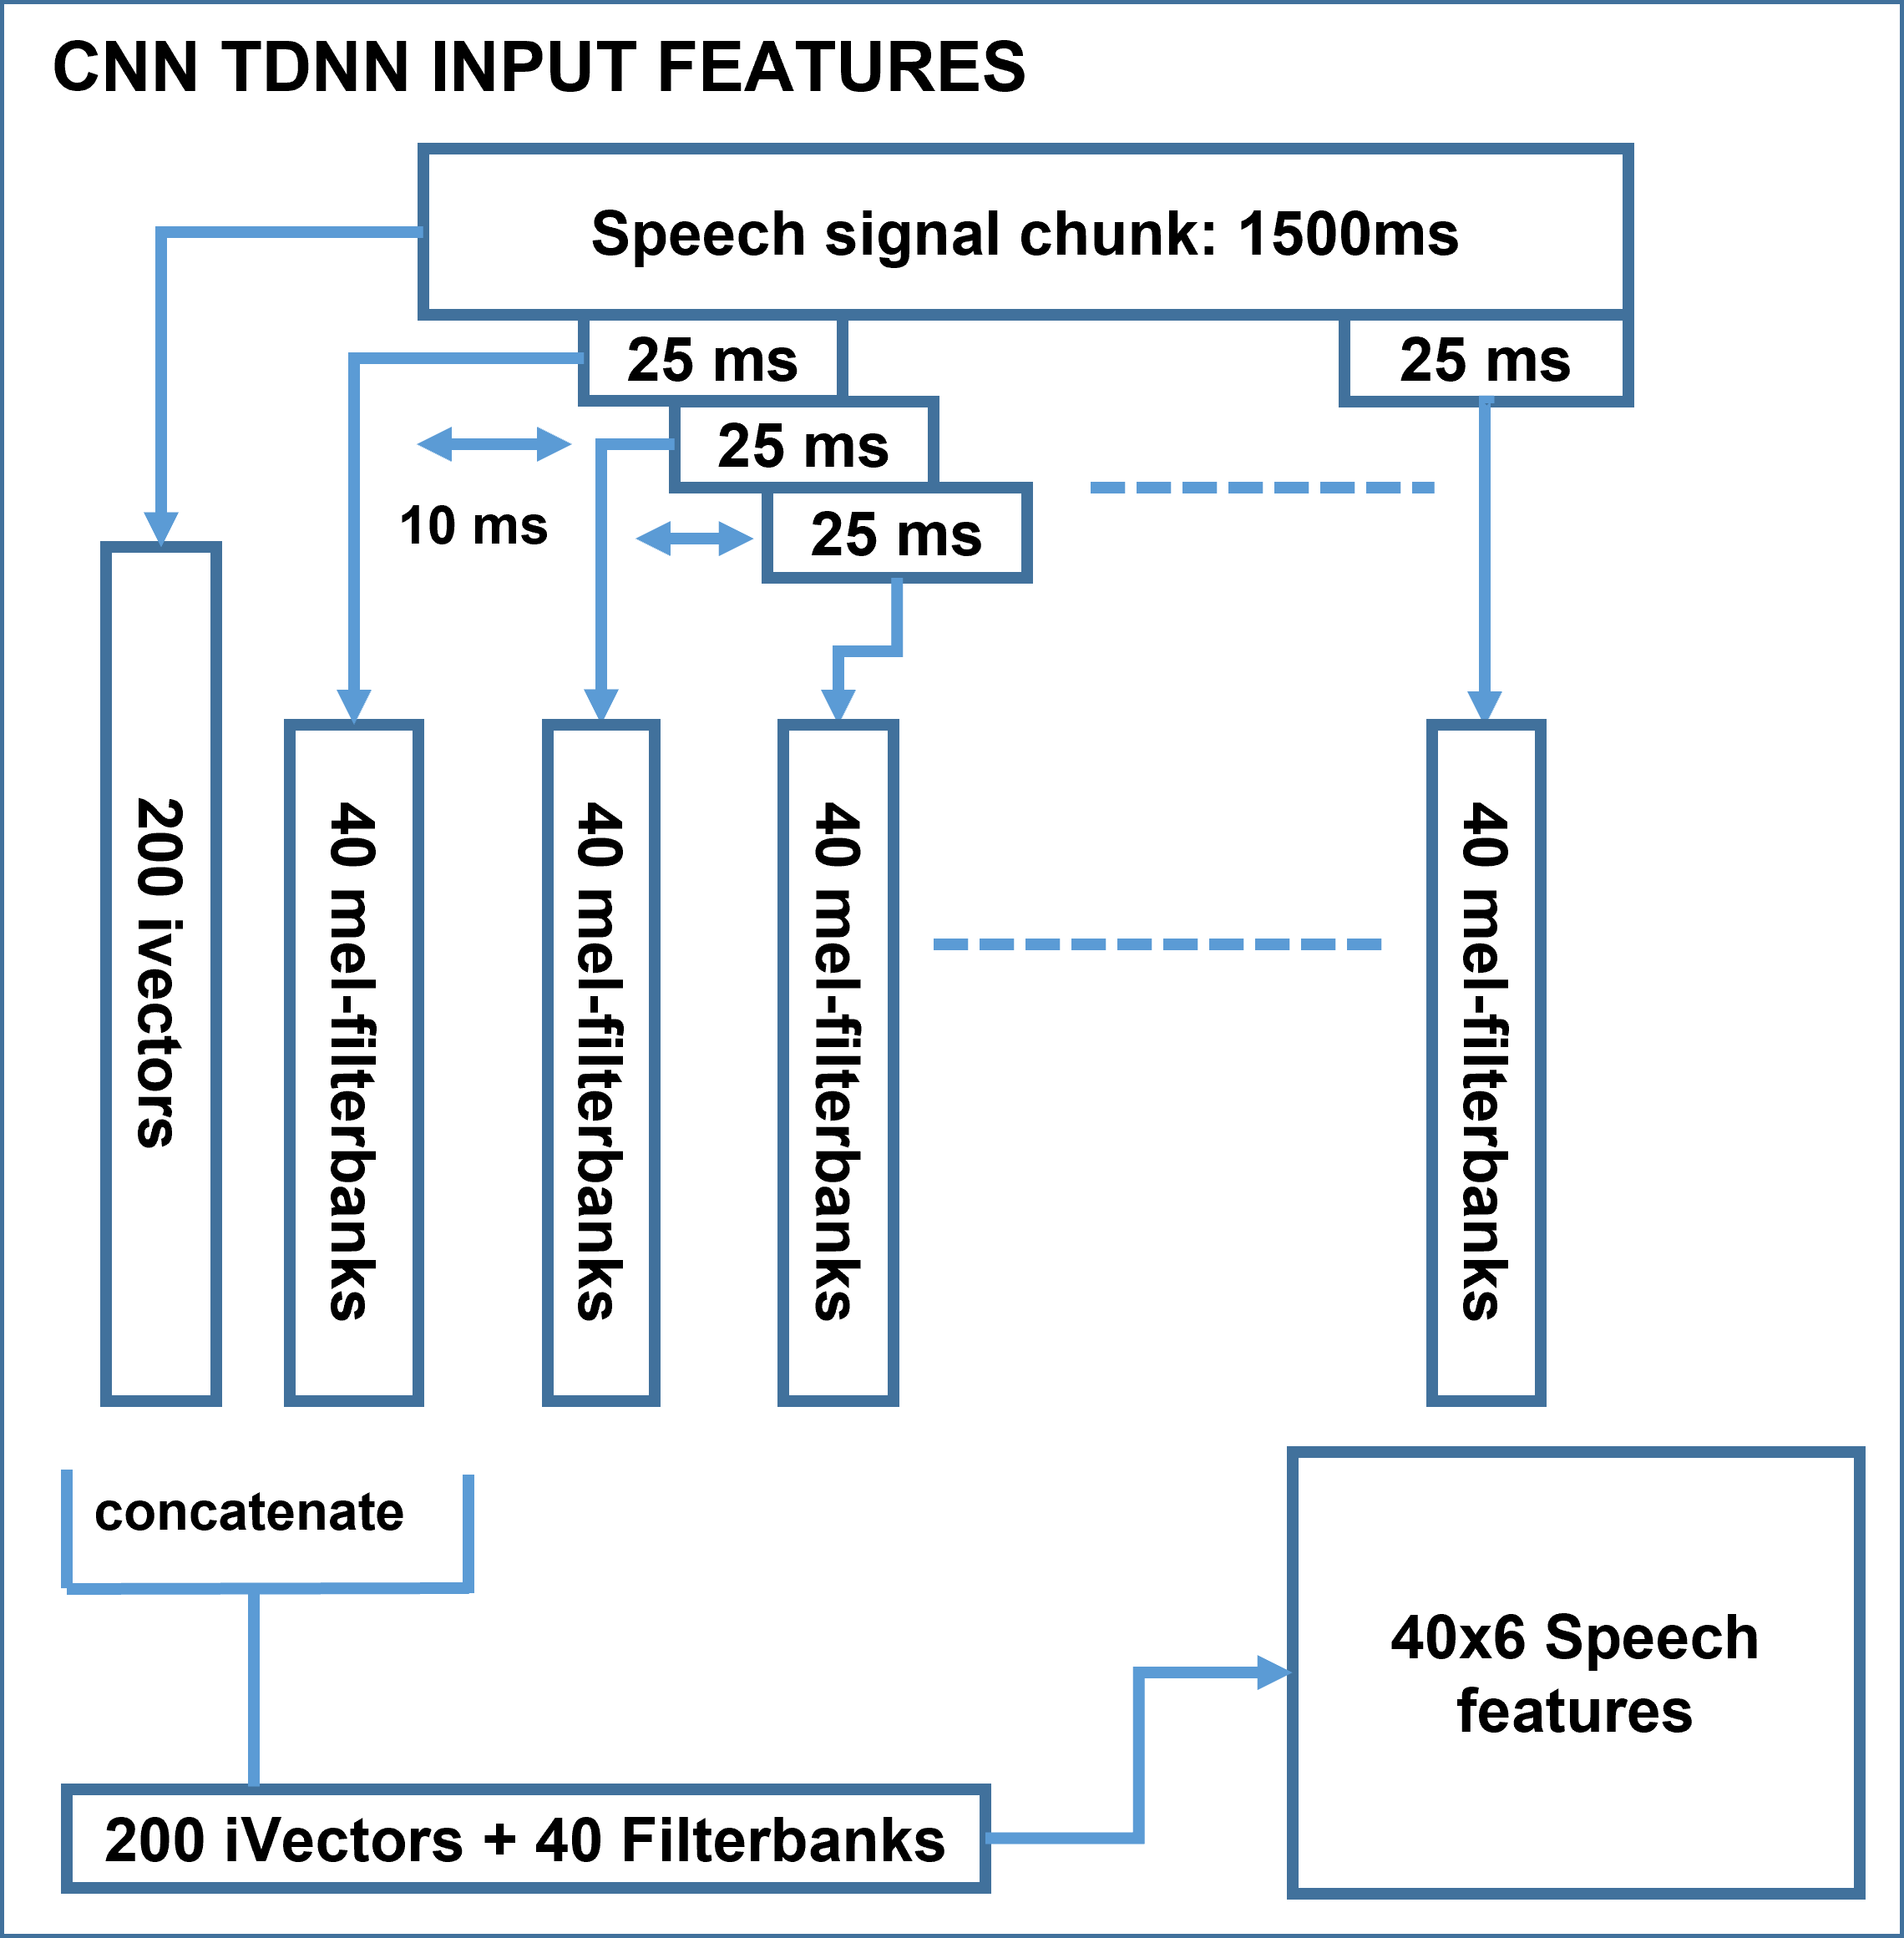
\includegraphics[width=0.4\textwidth]{img/CNNTDNN-INPUT.png}
    \caption{CNN-TDNN Input}
    \label{fig:CNN-TDNN-INPUT}
\end{figure}



\begin{figure}[h!]
    \centering
    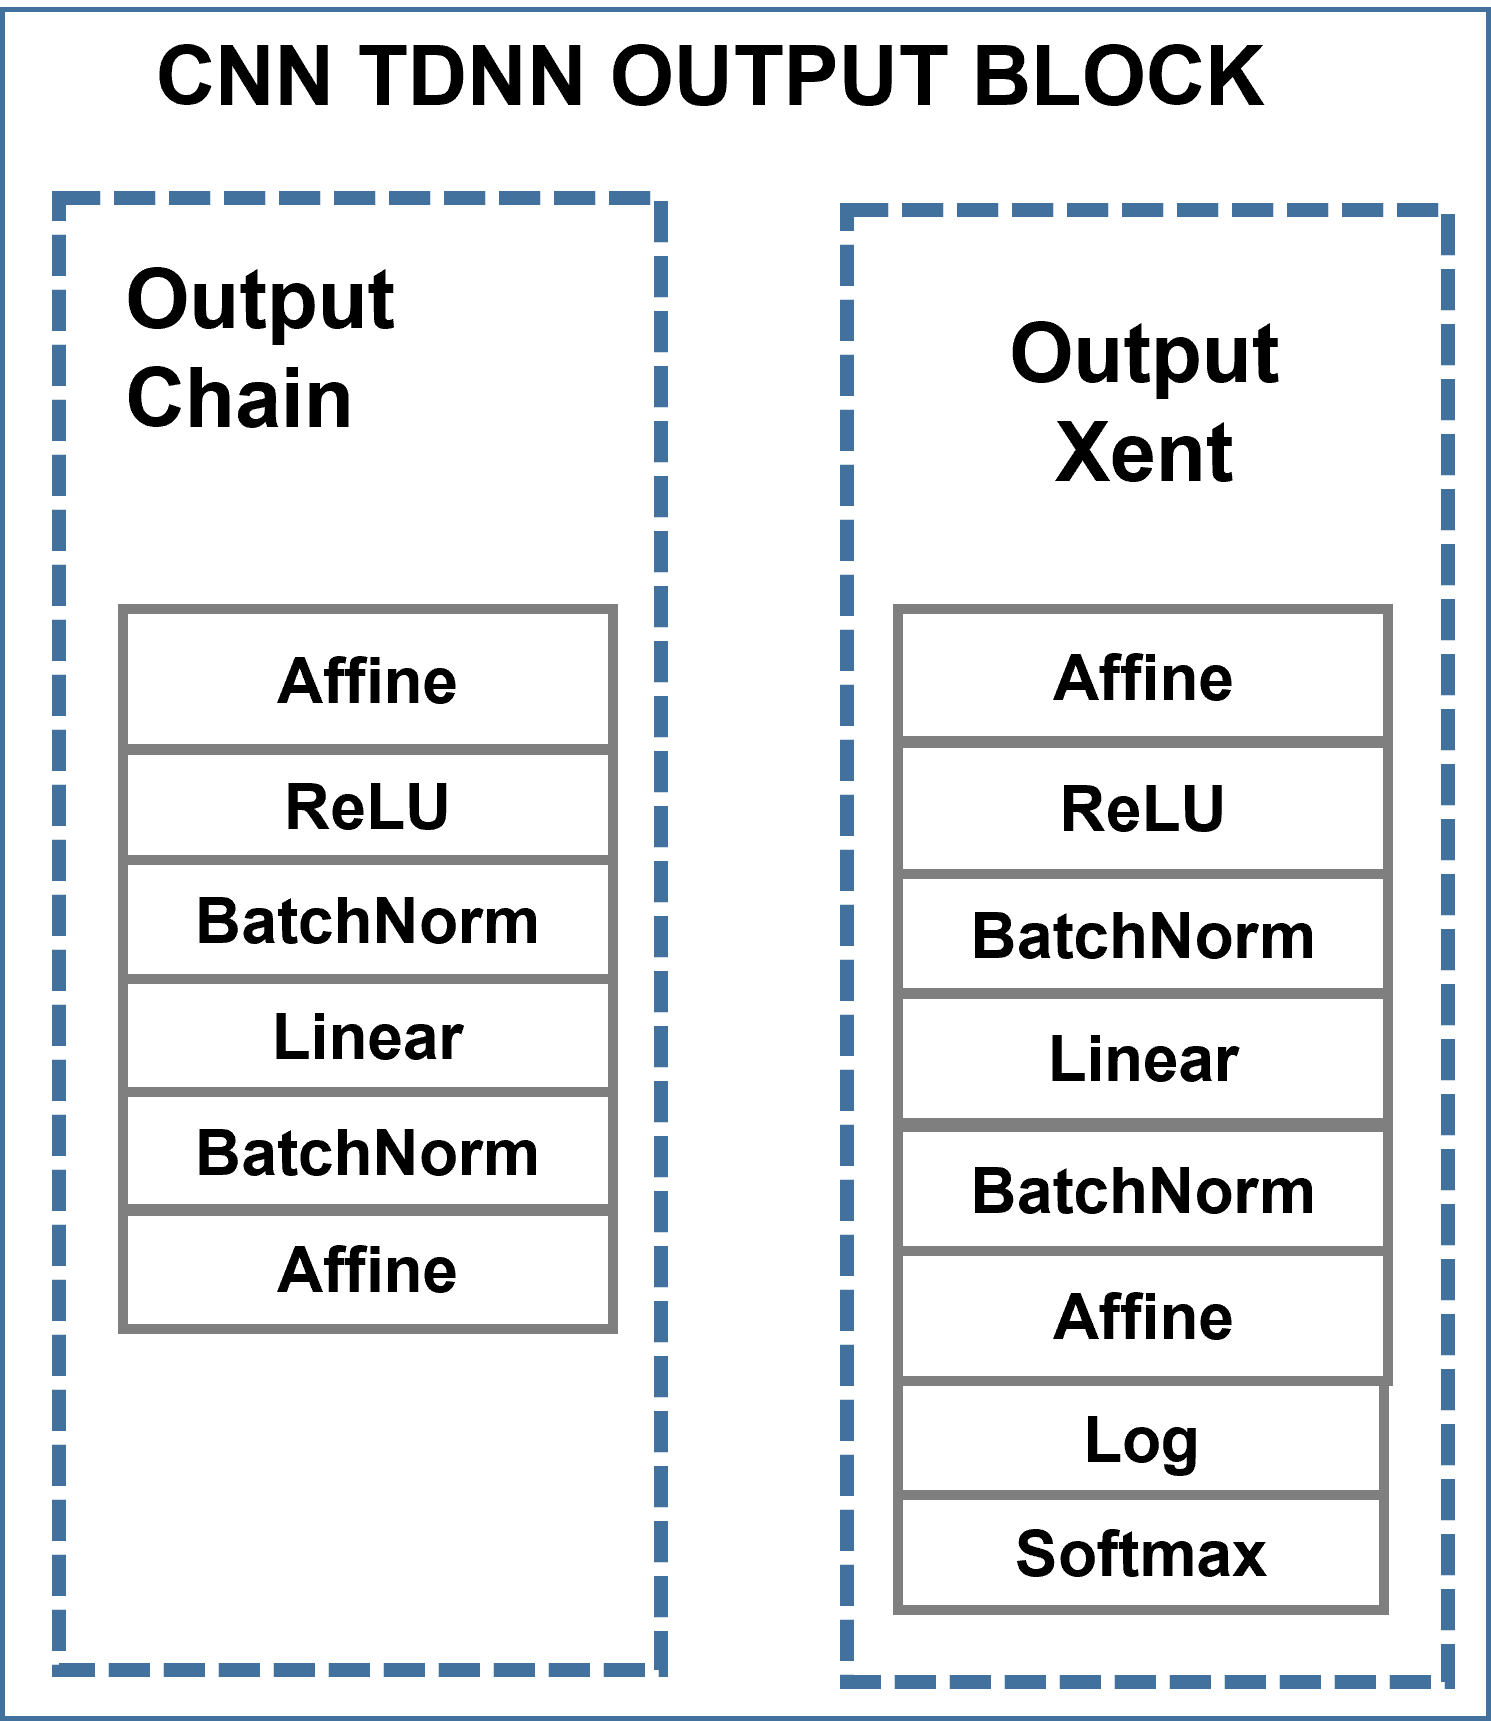
\includegraphics[width=0.3\textwidth]{img/CNNTDNNOUTPUT.png}
    \caption{CNN-TDNN Output}
    \label{fig:CNNTDNN-output}
\end{figure}

%Ghahremani \cite{ghahremani_acoustic_2016} proposed a CNN-TDNN-based raw waveform setup with a repeated network-in-network structure that aggregates time information from convolution filter outputs.

%It introduces Network in Network layer which is a group of micro neural network blocks applied to non-overlapping patches of input with each block being a nonlinear transformation from m dimensional space to n-dimensional space. NIN is a many-to-many non-linearity comprising of two block diagonal matrices, with repeated blocks, inter-leaved between layers of ReLU or Rectified Linear Units. To stabilize training we always add a normalization layer after the NIN non-linearity.

%If the micro neural network block parameters are shared across the NIN, each column of the block $U_{1}$ can be interpreted as a one dimension convolution filter with a filter size \textit{m} and a filter shift \textit{m}. Thus, the same filter is applied to non-overlapping patches and this models local connectivity. The shared parameters in the NIN non-linearity keeps its total parameter count low relative to the size of its input and output, and allows it to be trained faster \cite{ghahremani_acoustic_2016}.

%\begin{figure}[h]
%    \centering
%    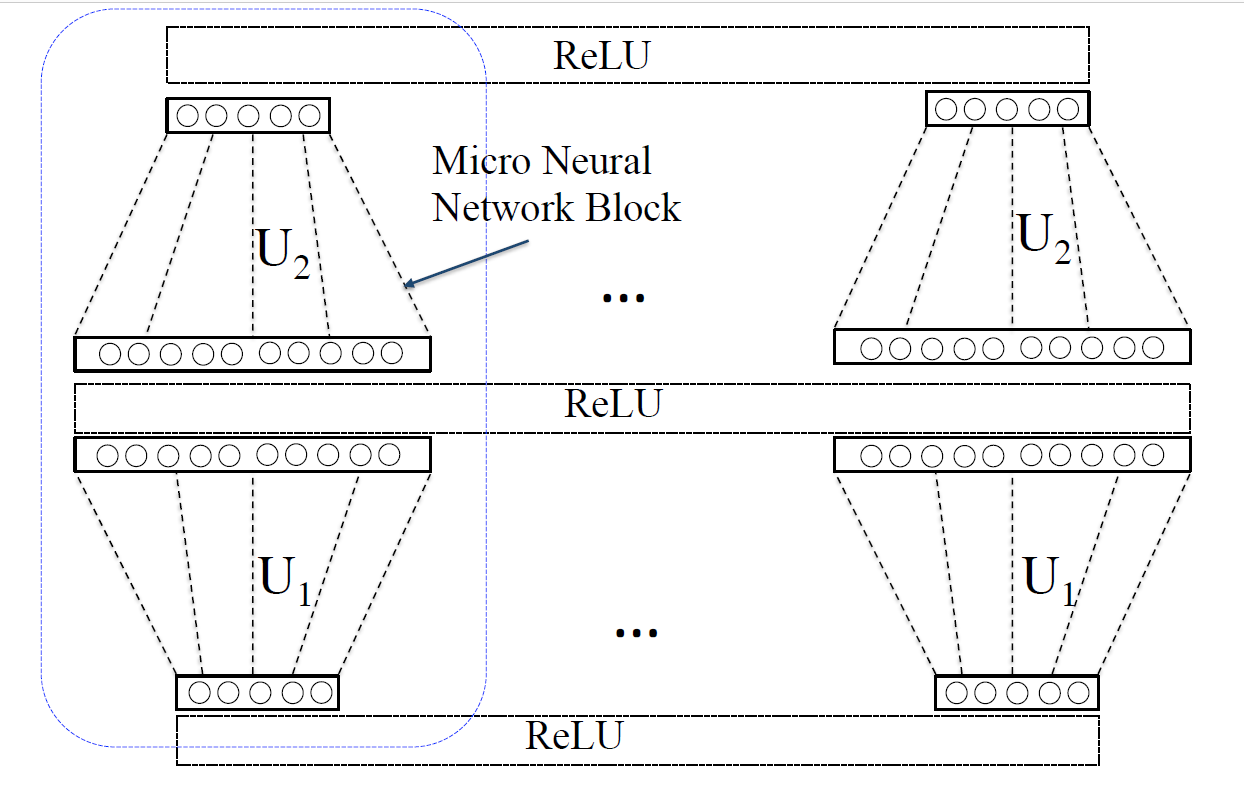
\includegraphics[width=0.6\textwidth]{img/NIN.png}
%    \caption{NIN structure}
%    \label{fig:NIN}
%\end{figure}

%If this Network In Network (NIN) non-linearity replaces the conventional ReLU hidden layer in the DNN, the results improve. 

\subsection{Using Maximum Mutual Information Model for HMM-DNN Systems}

Discriminative objective functions like Maximum Mutual Information (MMI) or Maximum Conditional Likelihood Estimation objective functions are trained to maximize the gap between the correct and incorrect answers, or to differentiate between right and wrong answers instead of assigning high weights values to the correct sequences which helps training model to improve the correct output sequence prediction, while making incorrect sequences less likely \cite{povey_purely_2016}. 

Deep networks excel in feature extraction and discovering correlation among them which allows exploitation of contents in making predictions. DNN can be used in ASR to classify phones based on the features extracted in acoustic frames. It is treated like a classifier using softmax to output the probability distribution $P(phone | x_{i})$. The softmax pulls up the ground truth while pulls down the others which is the same concept as Maximum Mutual Information Estimation \cite{wiesner_lattice_2020}.

\begin{equation}
 p_{i} = \frac{e^{score_{i}}}{\sum_{c \in y} e^{score_c}}
\end{equation}

Maximum Likelihood Estimation uses sequence training but it is not discriminative. The softmax function is discriminative here. The term Sequence means that the objective considers the entire utterance rather than "frame-level" objectives such as cross-entropy. The term discriminative refers to the use of an objective function that supposedly optimises some task-related criteria, and then directly minimising that objective using gradient-based methods \cite{noauthor_lattice_nodate}.

To turn MLE into a discriminative sequence training, the classifier is trained by minimizing the cross-entropy and the model is utilized to generate alignments and lattices which is called the discriminative training phase. 

The second phase is the sequence training. Since both the deep network and the lattice are network objects, they can be trained together. This model is then used to calculate the MMIE or Minimum Phone Error objective with the forward-backward algorithm followed by back-propagation to learn the model parameter \cite{wiesner_lattice_2020}.

MMI objective for ASR can be expressed as \cite{noauthor_lattice_nodate}:
\begin{equation}
    F_{MMI}(\theta) = \sum_{r=1}^{R} log \frac{P_{\theta}((O_{r}|M_{Wr})P(w_{r})}{\sum_{\hat{w}}P_{\theta}(O_{r}|M_{\hat{w}})P(\hat{w})} 
\end{equation}

Where $M_{w}$ is HMM that corresponds to transcription \textit{w}. To normalise the numerator, the objective function accounts for the log-probability of complete utterance in the numerator dividing it by the log probability of all possible utterances in the denominator. Thus, the distributions with the subscript $\theta$ are trained parameterized distributions \cite{wiesner_lattice_2020}.

%\begin{figure}[h]
%    \centering
%    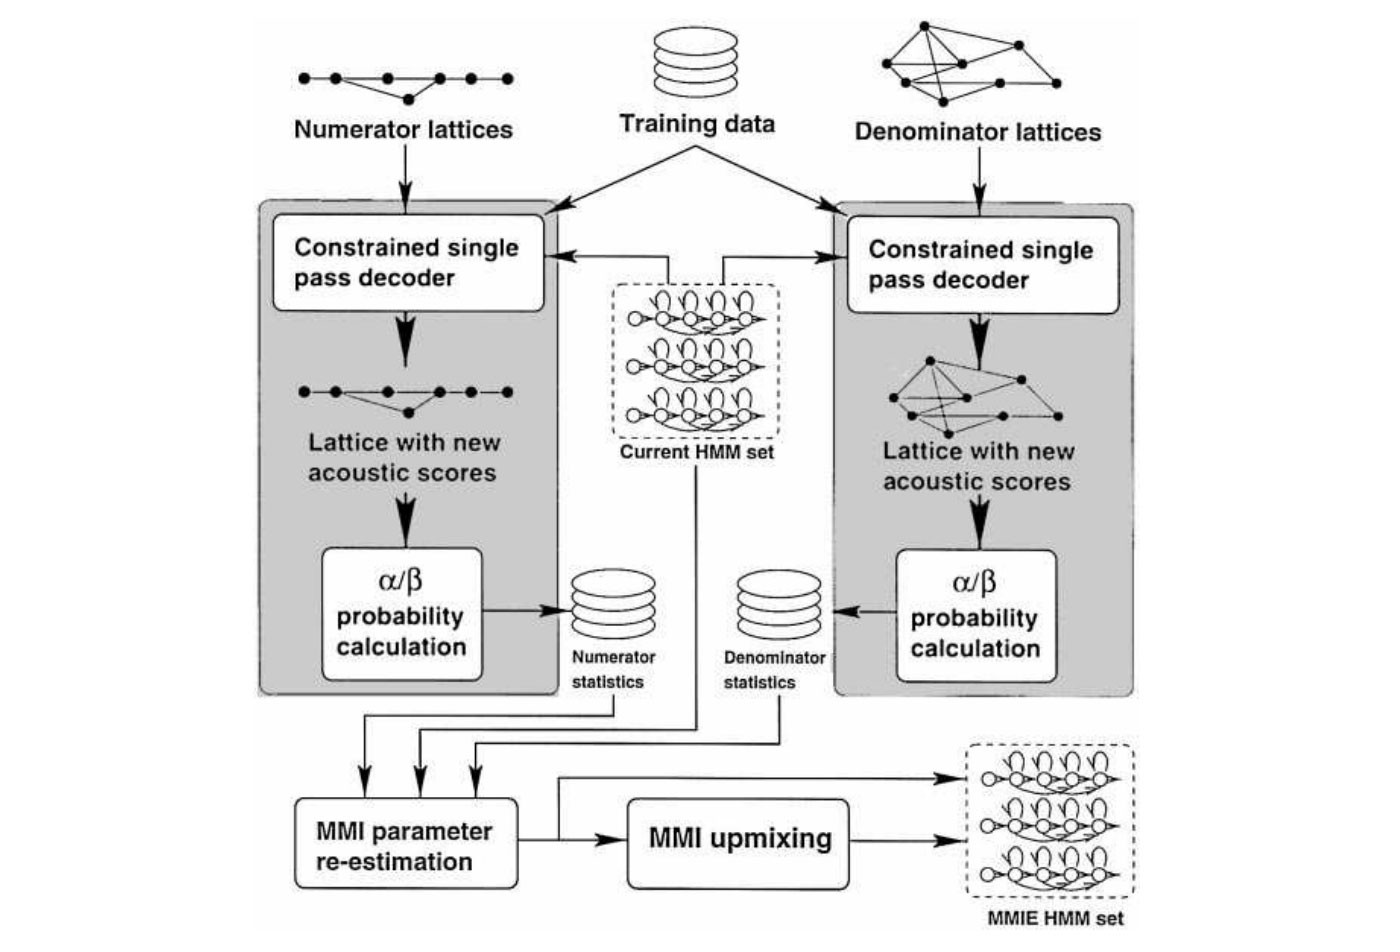
\includegraphics[width=0.9\textwidth]{img/LatticsbasedMMI.jpeg}
%    \caption{Lattice Based MMI system}
%    \label{fig:latt-based-mmi-sys}
%\end{figure}

MMI requires First order Gradient based methods for optimization, such as Stochastic Gradient descent, which requires knowledge of the gradient of the MMI objective with respect to the parameter $\theta$. The neural network function performs forward propagation, while back-propagation computes the corresponding gradient. The state occupancies for the numerator and denominator terms must be computed for the gradient overall objective \cite{daniel_povey_kaldi_nodate}.

Calculating the denominator sum requires summing over an exponentially large amount of word-sequences, which is impractical. Two methods can be used to approximate the sum \cite{noauthor_lattice_nodate}:

\begin{enumerate}
    \item \textbf{N-best list:} This less used and crude method of approximation is computed once and used for all utterances. 
    \item \textbf{Lattice structure:} It can be a word or phone based structure. A path through the lattice denotes a probable phone or word sequence. Lattices require initialization with a trained model which is a drawback, and cross-entropy trained systems are usually used for this purpose. 
\end{enumerate}

%\begin{figure}[h]
%    \centering
%    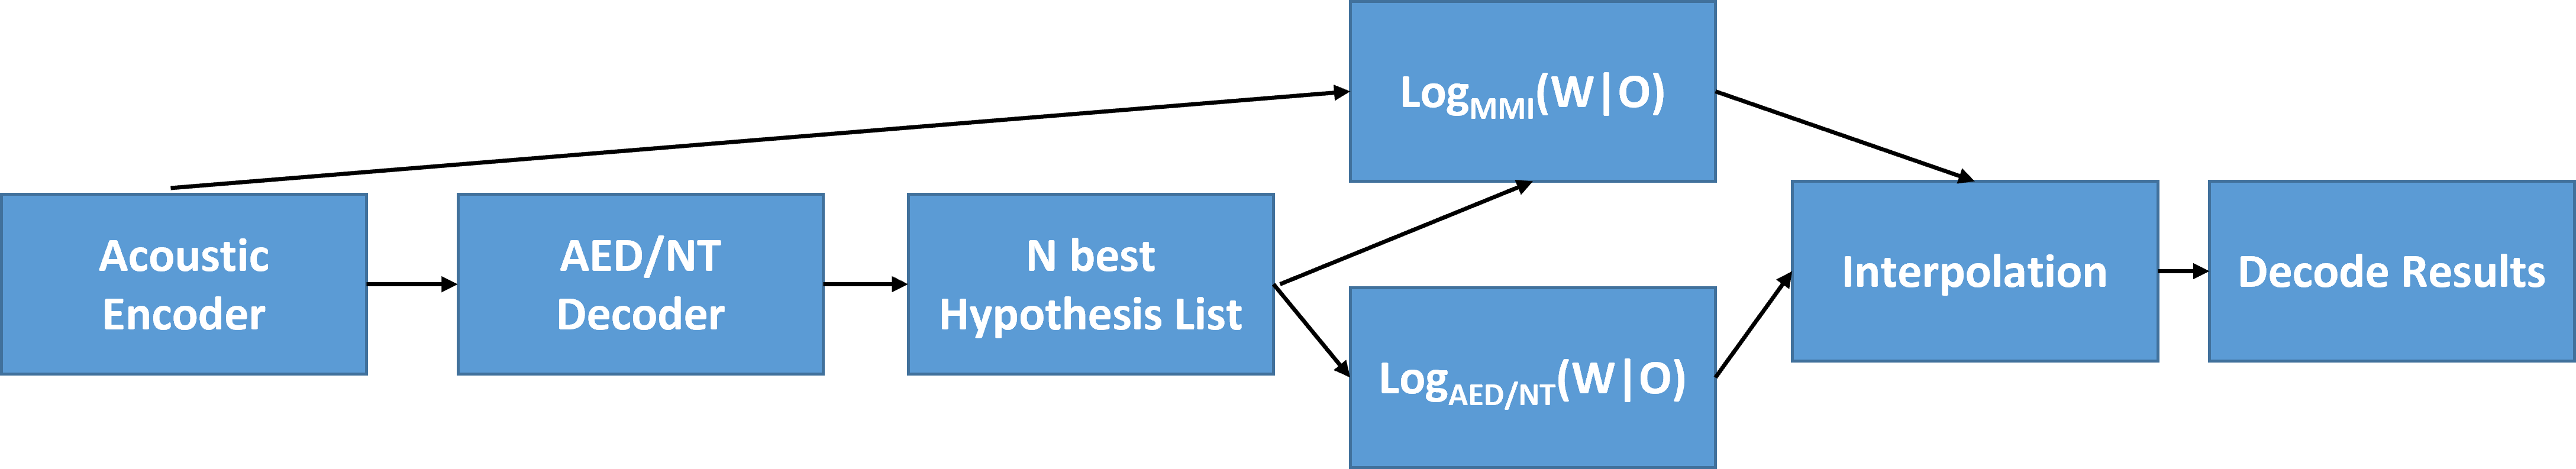
\includegraphics[width=0.9\textwidth]{img/MMISCORING.png}
%    \caption{MMI Scoring}
%    \label{fig:MMI-scoring}
%\end{figure}

The denominator in a lattice-based MMI is first identified by the word lattice. Classifying phones with Deep Learning requires pre-training a deep neural network with cross-entropy. The scaling fudge factor $kappa$ must also be used to correct the overestimation. While training a Deep Neural Network everything seems adhoc but this can be avoided \cite{wiesner_lattice_2020}.

%A composed transducer is generally used in Traditional ASR called H ◦ C ◦ L ◦ G to decode audio. It is a WFST and can be integrated with the deep network classifier. It is a big complex network which can be trained like DNN or DL using back-propagation without the requirement of introduction of a lattice for denominator approximation. Pdf-ids are numerical values of context dependent states given by decoding graphs formed by the decoding algorithms which uses WFSTs to provide graph operations used in acoustic modelling. WFST are used in HMM-GMM models and can also be used along with Deep Neural Network Classifiers.

Lattice-based methods were proposed prior to GPU era. It is not possible to train this deep network without a GPU but with Deep Learning in 2012 on GPUs, new possibilities emerged but the physical limitations, particularly, memory consumption problem remained. To fit the method into the GPU's memory, for example, we chop the training utterances into 1 to 1.5 second chunks which is not enough. GPU allows one GPU instruction to be run on multiple data sets one at a time. We must avoid branching to get the most benefit out of the GPU and pruned tree search does not seem so appealing with GPU which is why a smaller model is required \cite{povey_purely_2016}.

\subsection{Bypassing Lattices through Chain Model for \\ Improving Efficiency}
With the advent of E2E models, the need of a trained system for lattice initialization became a disadvantage of lattice-based MMI. Hence, comes the concept of Lattice Free MMI \cite{povey_purely_2016, ghahremani_investigation_2017} which is purely sequence trained requiring no no cross-entropy training as it does not use a lattice allowing it to exactly compute the sum instead of just approximating it \cite{noauthor_lattice_nodate}. The LF-MMI objective function is the modified form of MMI discriminative  objective function which enables ASR Training on GPU in HMM-DNN ASR Approach. 

The \textit{chain} or LFMMI models are a different form of HMM-DNN model. It uses Neural Networks \cite{daniel_povey_kaldi_nodate} which are a different point of design in the space of acoustic models compared to Traditional ASR models. It uses a three times smaller frame rate at the Neural Network output which reduces the computational requirements significantly in test-time, making decoding in real-time  much simpler. 

Due to the reduced frame rate, unconventional HMM topologies must be used to enable one-state HMM traversal. The chain model employs HMM's fixed transition probabilities but does not train it actually. Neural-net output probabilities can typically serve the same purpose as transition probabilities depending on the topology \cite{daniel_povey_kaldi_nodate}.

Models are trained with a sequence-level objective function, i.e. the log-probability of the correct sequence, from the start. It is implemented in an MMI-based system without lattices on GPU by performing a complete forward-backward computation on a decoding graph derived from a phone-based n-gram language model \cite{povey_purely_2016}. 

\begin{figure}[h]
    \centering
    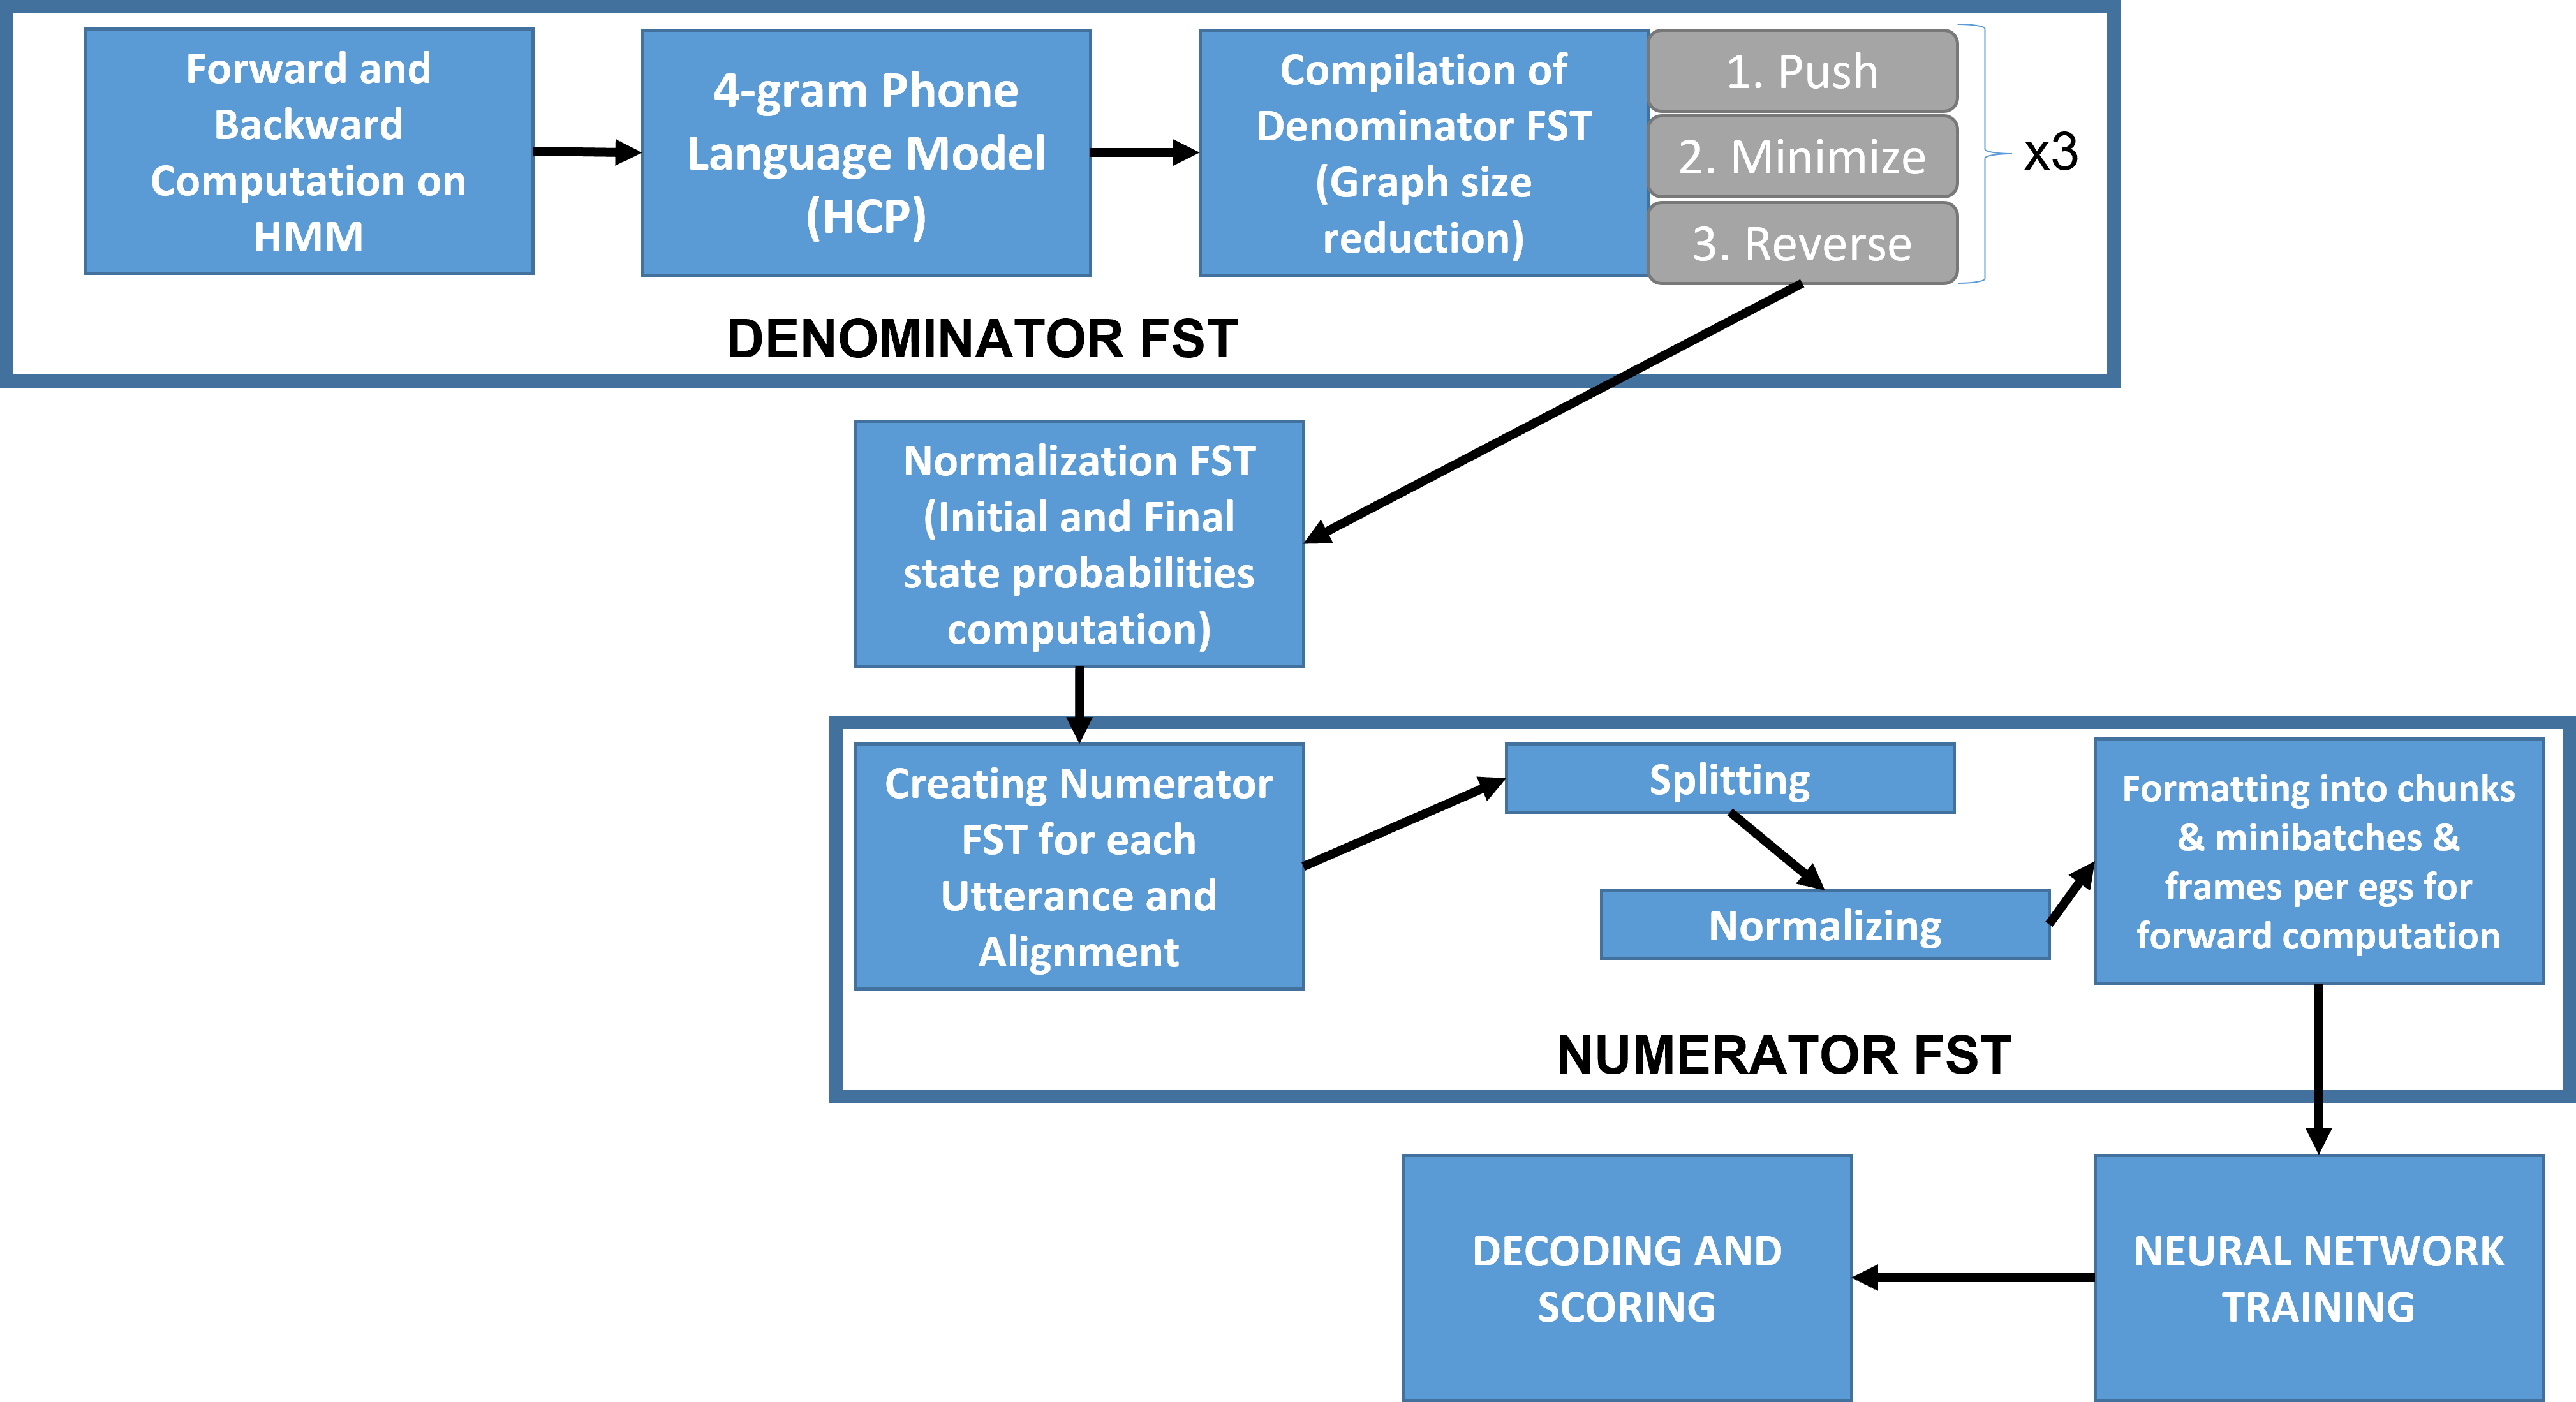
\includegraphics[width=0.45\textwidth]{img/ChainTrg.png}
    \caption{Chain Model Overview}
    \label{fig:chain-overview}
\end{figure}

%https://slideplayer.com/slide/17724439/
%https://jonathan-hui.medium.com/speech-recognition-maximum-mutual-information-estimation-mmie-a0db565764aa

If the denominator is represented as a graph and it is fitted in the GPU allowing computations to be efficiently performed for which following modifications are done \cite{noauthor_lattice_nodate, wiesner_lattice_2020}:

\begin{enumerate}
    \item Using Phone LM instead of Word-based LM to reduce size of graph significantly because there are far fewer possible phones than there are words.
    \item There are three times fewer outputs for any utterance to compute because DNN outputs are computed at a third of the standard frame-rate \cite{povey_purely_2016} which is done by decreasing the frame-shift to 30ms from traditional 10ms which means that the standard 3-state left-to-right HMM topology, commonly used in ASR, cannot be used since the entire HMM is required to be traversed in a single frame. Training such a system using the MMI objective requires the objective and its derivative to be computed effectively. 
    
\end{enumerate}

We have very limited transcribed data available for training purposes but we do have a huge amount of Call Center Data available. If we only have only a small amount of data transcribed, but much more un-transcribed data best is to train a seed model and use it to transcribe more data. But also don't want to train further on incorrect captions. So we apply data filtering based on confidence scores to select out the harder data that is most useful for refining the system. One of the solutions can be \cite{ghahremani_investigation_2017} to use a lattice to incorporate uncertainty about the transcription, and train with the LF-MMI criterion but that requires a strong language model for the best performance\cite{wallington_learning_2021}.

LF-MMI has shown to achieve better performance on various data-sets like Aspire using various different HMM-DNN and E2E ASR frameworks \cite{ghahremani_investigation_2017, tian_consistent_2022} compared to lattice based MMI model.




%For instance, Arabic Language has a base word which comprises of three letters. E.g.     \makeatletter\bgroup\beginR\fontencoding{LAE}\selectfont علم\endR\egroup (pronounced as Ilm) means knowledge. This is the base word. The word \makeatletter\bgroup\beginR\fontencoding{LAE}\selectfont معلم\endR\egroup (pronounced as Mualim) means teacher or mentor, the connotation means transmitter or sharer of knowledge. The essence and the characters or alphabets of the base word \makeatletter\bgroup\beginR\fontencoding{LAE}\selectfont علم\endR\egroup (comprising of 3 alphabets "\makeatletter\bgroup\beginR\fontencoding{LAE}\selectfont ع \endR\egroup" "\makeatletter\bgroup\beginR\fontencoding{LAE}\selectfontل\endR\egroup" "\makeatletter\bgroup\beginR\fontencoding{LAE}\selectfontم\endR\egroup") remains there as the word compounds and expands. If this structure is learned by the Computer through Machine Learning, Machines may be able to capture out-of-vocabulary words more easily. 

%All morphology-based approaches aim to decrease ASR errors by lowering the OOV rate through modelling at the morph level and also account for the lack of wide-vocabulary data since we are not always able to arrange an audio data-set for each and every word that might be found in the dictionary. In morph-based language modelling, morphs are used in place of words, but because multiple morphs are related to a single word, the context may need to be longer. \cite{creutz_morph-based_2007}.

%Morfessor is an unsupervised data-driven method for the segmentation of words into morpheme-like units.It Aims to identify frequently occurring substrings of letters within either a word list (type-based) or a corpus of text (token-based). It uses a probabilistic framework to balance between few, short and many, longer morphs. 
%[http://morpho.aalto.fi/projects/morpho/]